% uplatex dmrhow2
% uplatex dmrhow2
% dvipdfmx dmrhow2

\documentclass[a4j,oneside]{ujbook}
\usepackage[schinese,japanese]{pxbabel} % \foreignlanguage{schinese}{}
\usepackage[dvipdfmx]{graphicx} % \includegraphics{}
\usepackage{bmpsize}
\usepackage[dvipdfmx]{hyperref} % \url{}
\usepackage{pxjahyper} % 日本語しおり ※hyperref → pxjahyper の順であること
\usepackage{enumitem} % \begin{description}[nextline]
\usepackage{ascmac} % \yen
\usepackage{here} % [H]
\begin{document}

\title{DMR 始めました}
\author{JG1UAA (uaa@uaa.org.uk)}
\西暦 % TeX Live 2018 は令和に対応していない (2019.4に発表されたから仕方ない)
\date{\today}

\maketitle
\tableofcontents

\chapter{はじめに}

\section{DMR って何}

Digital Mobile Radio の略で、ETSI (European Telecommunications Standards Institute 欧州電気通信標準化機構) により制定されたデジタル無線機の規格です。既に日本国内では D-STAR や C4FM といった方式のデジタル対応アマチュア無線機が販売されていますが、DMR はアマチュア無線だけではなく業務用機、dPMR と呼ばれるラインセンスフリーの無線機と幅広く使われています (ただし、海外で)。

\section{D-STAR/C4FM と何が違うの}

DMR もデジタル無線機なので、音声を量子化 (サンプリング) →圧縮やエラー訂正符号を付加→デジタルデータを RF モデムを通じてやりとり、という手順は変わりません。音声の圧縮処理に使われるボコーダーは C4FM と同じ AMBE+2 で、変調方式/変調速度も C4FM と同じ 4 値周波数偏位変調/9600bps です。ただし DMR は時分割多元接続 (TDMA) により一つの周波数で二回線の通信を可能にしている点が違います。また、インターネットを使用した中継 (VoIP) も BrandMeister や DMRplus ネットワークを使用し、簡単に行うことが可能です。

\section{どういう人に向いていないか}

最初に厳しいことを書きますが、以下の項目に該当するのであれば DMR ではなく他のデジタル方式のアマチュア無線機をお勧めします。
\begin{itemize}
 \item 英語を目にするのも嫌だ
 \item 日本ブランドでないものは買いたくない
 \item メーカーサポートが充実していないと不安だ
\end{itemize}
海外発祥の規格ですし、無線機も海外産、なので購入する際のやりとりは英語が基本です。また情報も日本より海外に多いため、必然的に英語が分からなければ困ることが多いです (最近では日本語での情報も増えてきましたが)。海外から無線機を個人輸入する以上、故障などのトラブルが発生した場合の対処も自分で何とかしないといけません。
\begin{itemize}
 \item JARD や TSS にお金を払うのは嫌だ
 \item 送信機系統図を書くのは面倒だ
\end{itemize}
海外産の無線機を使う以上、技適なんてものは当然ありません。なので送信機系統図を書き、JARD や TSS を利用して保証認定を取る必要があります。
\begin{itemize}
 \item Linux やネットワーク (インターネット) には触りたくない
\end{itemize}
DMR 機同士で直接シンプレックス通信をする場合は問題にならないのですが、Pi-Star 等のホットスポットを用意して VoIP 越しに通信する場合は Linux やネットワークに関する知識が必要になります。コマンドラインによる Linux の操作ができないと困りますし (本書には VMware による仮想環境に Linux をインストールして簡単なホットスポットを作る話があります)、ネットワークについても無線 LAN ルータを設定できる程度の知識は必要でしょう。

\section{どういう楽しみ方があるか}

無線機である以上、同じ形式の無線機を用意して「誰か」と話すことは可能です。シンプレックス通信でどこまで届くかというのも立派な実験になりますが、DMR は D-STAR/C4FM よりも (日本国内では) マイナーな方式なため、現状では通信相手を探すことが容易ではありません。なので、多くは Pi-Star 等のホットスポットを用意し、BrandMeister 等のネットワーク越しに会話をするような使い方が主体になります。

日本国内では誰も使っていないような海外製の無線機を、どうにかして日本の法の下で合法的に使うという挑戦もあります。無線機を分解することで現在のテクノロジがどこまで進んでいるかを知る機会になりますし、自分の手で送信機系統図を書いた無線機で申請して手にした免許状は一段と愛着の持てるものになるかもしれません。

Pi-Star 等のホットスポットを構成するソフトウェアは、オープンソースのものが多いです。腕に覚えのある方は、ソフトウェアの改良や (Linux 以外の OS、例えば *BSD 等への) 移植を行い、作者へフィードバックするのも良いでしょう。

無線機そのものを自作して運用するということが困難になってきた時代ではありますが、既製品とソフトウェアを組み合わせ、自分なりのシステムを構築するという余地が DMR にはまだ残されています。

\chapter{最初に必要なのは DMR ID}

\section{ID が無いと始まらない}

DMR の世界では、7 桁の ID (DMR ID) がコールサインの代わりとなります。この ID が無いと何も始まらないので、\url{https://www.radioid.net/register} へアクセスし、ここから画面の指示に従って操作を行えば取得できます (日本語のページは今のところありません)。
\begin{figure}[H]
 \centering
 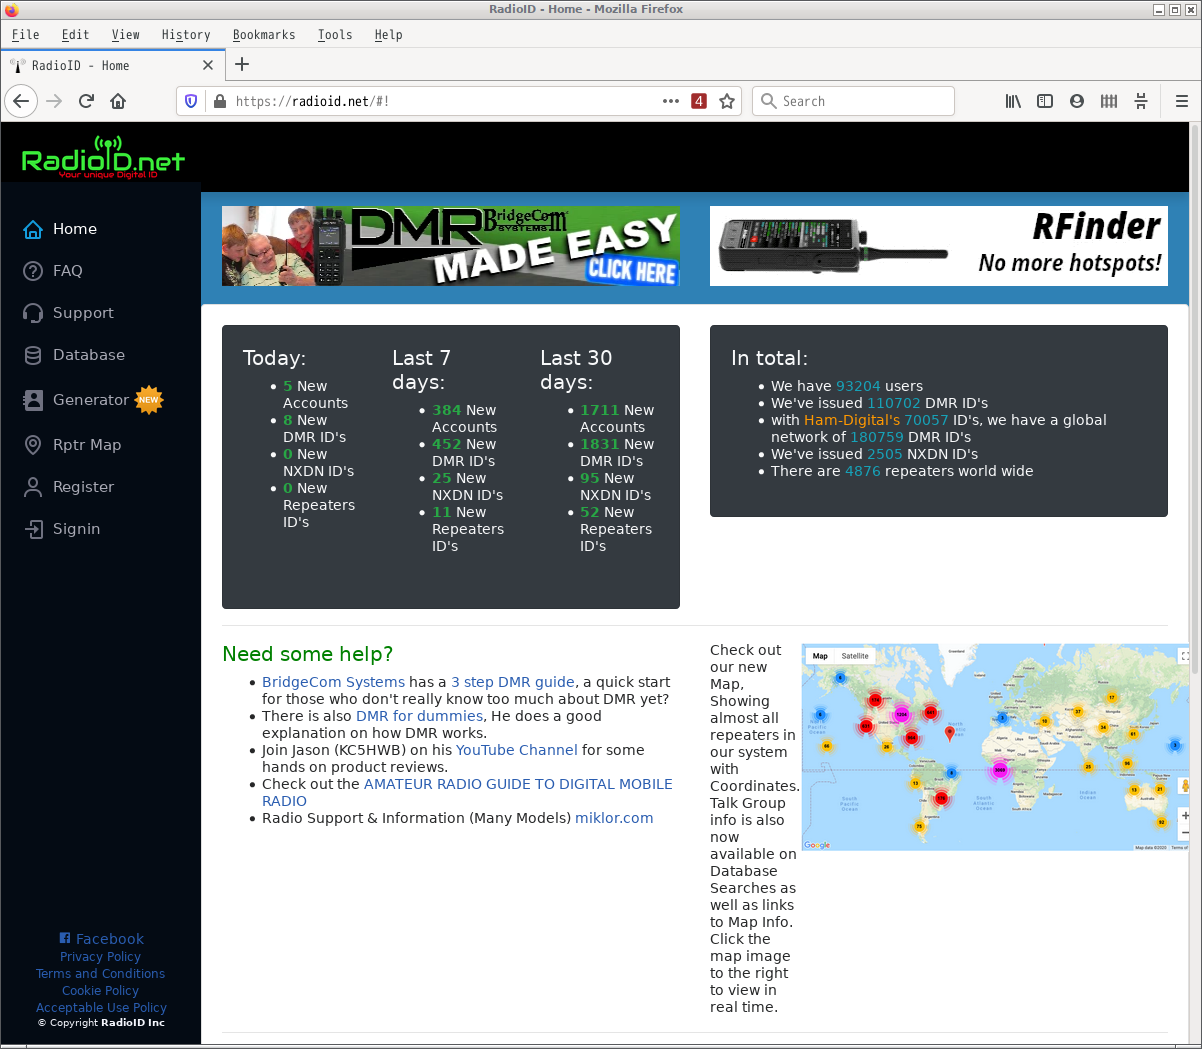
\includegraphics[width=15cm]{img/radioid_net2.png}
 \caption{radioid.net のトップページ}
\end{figure}
DMR の無線機とホットスポットを運用する場合、機材は二つありますが ID は一つあれば問題ありません。同じ ID を両方の機材に設定して使うことになります。

DMR ID を手にできれば最初のステップは終了です。次に無線機を手にしましょう。

\chapter{無線機を買う}

\section{どこで何を買うのか}

DMR 対応のアマチュア無線機は色々ありますが、初めて購入するのであればユーザ数と情報の多い TYT MD-380 (UHF) 一択です。この機種は当然ながら技適が無いため送信機系統図を書いて JARD や TSS による保証認定を受ける必要がありますが、スプリアス発射強度に関する情報を (少なくとも JARD は) 持っているようで、こちらで測定データを用意する必要がありません。

MD-380 はいわゆる「洋モノ無線機」であるため日本国内では販売されておらず、基本的には eBay や AliExpress 等の海外通販サイトから購入することになります。最近では amazon.co.jp でも扱われていることがあるようですが、購入できたとしてもその後の扱い (設定方法や使い方) を調べるには英語が必須となるので注意してください。

MD-380 は「MD-380 walkie talkie」等のキーワードで検索できますが、購入する際は以下の二点に注意してください。
\begin{itemize}
 \item プログラミング用ケーブル (Programming Cable) が添付されていること
 \item AC アダプタが US 仕様であること
 \item UHF (430MHz) モデルであること
\end{itemize}
プログラミング用ケーブルは別途購入することも可能ですが、セットで買った方が面倒が少ないです。また、MD-380 は UHF (430MHz) モデルの他に VHF (144MHz) モデルもありますので、間違えないようにしてください\footnote{厄介なことに、MD-UV380 というよく似た名前の無線機もありますが、これは別物です。MD-380 が入手できなかった場合は OEM の Retevis RT3 (RT3S ではない) を使う手段もあるものの、この機種で免許が下りた実績があるかどうかは不明です。}。

筆者は 2018 年 8 月末、eBay にて \yen10k 程度の値段で購入しています。2021 年 7 月時点では eBay ではあまり見かけなくなってきており、AliExpress では \yen12k 程度で出ているようです。不当に安いものは詐欺の可能性があるので注意してください。なお、eBay はショッピングサイトではなくオークションサイトなので、ここで買い物をする場合は「Buy It Now」と Condition に「New」の設定を有効にしてから探すと良いでしょう。
\begin{figure}[H]
 \centering
 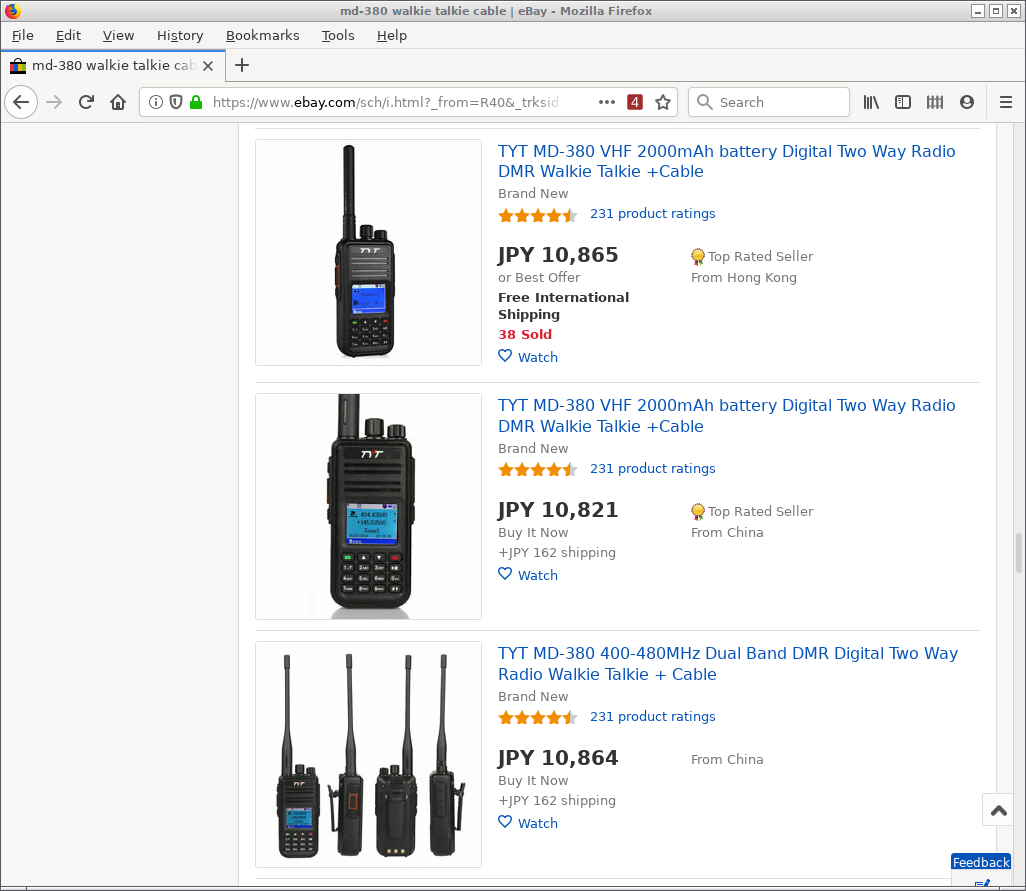
\includegraphics[width=15cm]{img/md380-ebay.png}
 \caption{eBay で売られていた TYT MD-380 の例}
\end{figure}
MD-380 を素直に買うのが面白くないと思うのであれば、適当な DMR 機を入手→分解して内部を解析し送信機系統図を作成→JARD の測定器室でスプリアス発射強度に問題がないことを確認し保証認定を受ける→免許申請、という手順もあります。実際、筆者は Retevis RT80 という DMR 機をこの方法で利用可能にしています。

\section{免許申請について}

先程書いたように TYT MD-380 (UHF) は技適が無いため、JARD や TSS による保証認定を受けた上で免許申請を行うことになります。無線局免許状の申請に必要となる、送信機系統図等の情報は、JQ1BWT さんの「DMR (Digital Mobile Radio)/D-STAR REFLECTOR の構築」(\url{http://www.bwt.jp/wiki/?DMR_Reflector}) や、Brand Meister の TalkGroup/44130 フリートーク DMR 勉強会 (\url{https://wiki.brandmeister.network/index.php/TalkGroup/44130}) にあるものが良いでしょう。他にも、「MD-380 送信機系統図」辺りのキーワードで Google 検索 (\url{https://www.google.com/search?q=MD-380+%E9%80%81%E4%BF%A1%E6%A9%9F%E7%B3%BB%E7%B5%B1%E5%9B%B3}) すれば見つけることができます。心配な方は回路図も GitHub (\url{https://github.com/pchickey/md380-re/tree/master/datasheets}) にありますから、提出する前の送信機系統図と一度比較してみてください。

工事設計書に記載する事項は、以下のようになります (電子申請 Lite 向けです)。
\begin{description}[style=nextline]
 \item[発射可能な電波の形式及び周波数の範囲] F2D F3E F7W 430MHz 
 \item[変調方式] F2D, F3E 上記以外の周波数変調 \newline
   F7W 四値周波数偏移変調 
 \item[終段管 (名称×個数・電圧)] RD07MUS2B × 1 個 7.4V 
 \item[定格出力] 5W
\end{description}
希望する電波の型式は 4VA、希望する空中線電力は 10Wです。

Web page によっては以下のような書類を同封・添付するようにという記述もあるようですが、筆者が 2018 年 8 月末に JARD を経由して免許申請を行った際はこれらは全て不要でした\footnote{オフバンド運用をしない誓約書・オフバンド不能化改造の証明は、おそらく Baofeng UV-5R が流行した 2010 年代前半の習慣の名残と思われます。少なくとも筆者は TYT MD-380 の変更申請 (増設) に際してはこれらの書類を出さずとも免許を受けることができておりますし、上にも書いた通りオフバンド運用をしないのは当然の義務である以上、このような書類は\underline{求められない限りは絶対に提出してはいけない}と筆者は考えています。}。
\begin{itemize}[style=nextline]
 \item オフバンド運用をしない旨の誓約書
 \item オフバンド運用不能化改造の内容およびそれを行った旨の証明
 \item 無線機に使用されているチップのデータシート
 \item 無線機の諸元
\end{itemize}
TYT MD-380 による申請が多いため、JARD や関東総合通信局が今のところはあまり細かいことを言わないだけという可能性は高いかもしれません。誓約書の有無に関わらず\textbf{オフバンド運用をしないのは当然の義務}ですから、阿呆な運用をして自らの首を絞めることがないよう注意してください。

\chapter{ホットスポット用 RF モデムボード (JumboSPOT) を買う}
\section{どこで何を買うのか}

ホットスポット用 RF モデムボードは色々あり、乱暴に分類するとこんな感じでしょうか。
\begin{description}[style=nextline]
 \item[MMDVM] 6cm × 5cm くらいの大きさのボードです。Raspberry Pi (Zero以外) に向いています。
 \item[ZUMspot/JumboSPOT] 6.5cm × 3cm くらいの大きさのボードです。Raspberry Pi Zero に合わせたサイズですが、Zero 以外のRaspberry Pi でも使用できます。
 \item[DVMEGA] 6cm × 4cm くらいの大きさのボードです。Raspberry Pi (Zero以外) に向いています。MMDVM よりも制御用マイコンが目立ちます。
\end{description}
どれも RF モデムとなる ADF7021 と、これを制御するためのマイコン (DVMEGA は ATMEL AVR、他は STMicro STM32) が搭載されています。今回は ZUMspot のクローン (コピー?) とも言われる JumboSPOT、それもアンテナと USB コネクタを装備して USB 対応ファームウェアが書き込まれたものをパソコンに繋いで使用します。

\begin{figure}[H]
 \begin{minipage}[t]{0.5\hsize}
  \centering
  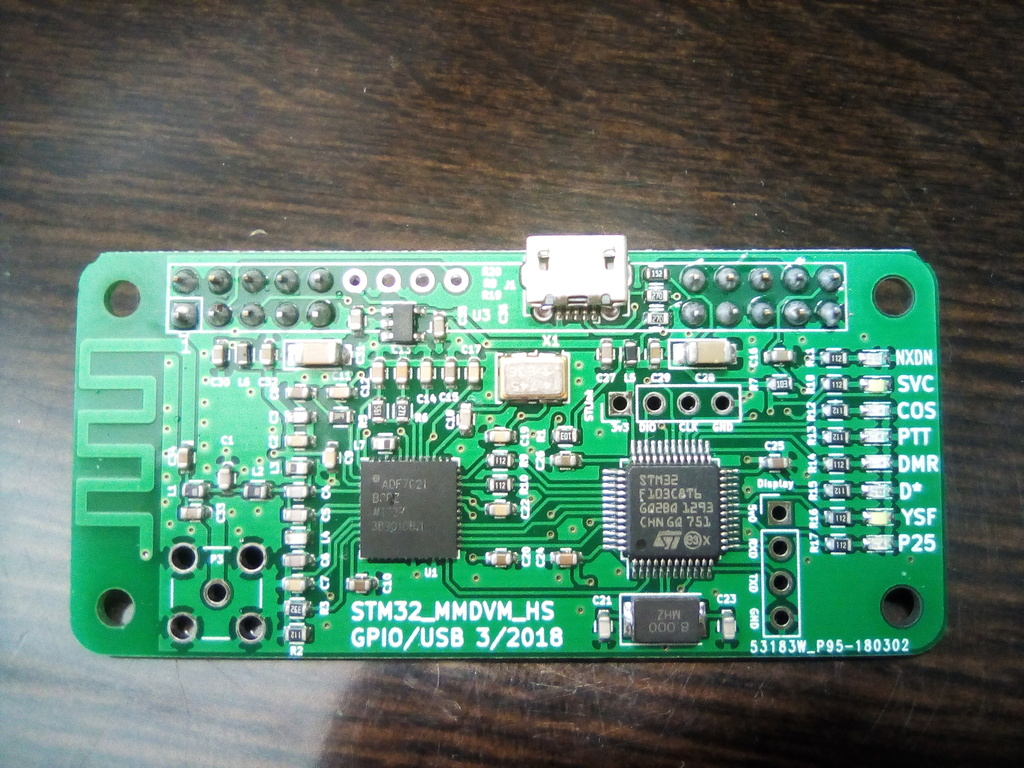
\includegraphics[width=6cm]{img/img_20190403_133143.jpg}
  \caption{JumboSPOT (表面)}
 \end{minipage}
 \begin{minipage}[t]{0.5\hsize}
  \centering
  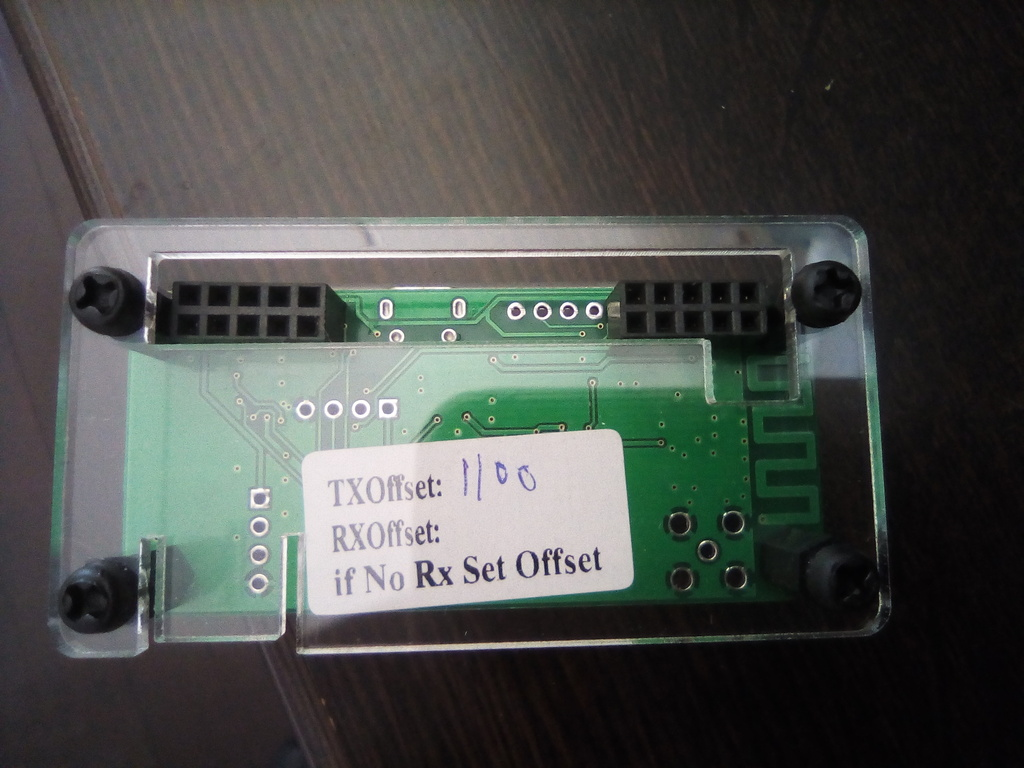
\includegraphics[width=6cm]{img/img_20190619_093448.jpg}
  \caption{JumboSPOT (裏面) \newline ※ Raspberry Pi Zero 用ケースを装備しています}
 \end{minipage}
\end{figure}

筆者は 2019 年 5 月中旬に、AliExpress の KaisayaHIFI audio Store (\url{https://www.aliexpress.com/store/939205}) という店から \yen2.5k 程度で購入しているのですが、その後は取り扱いを止めてしまっているようです。
\begin{figure}[H]
 \centering
 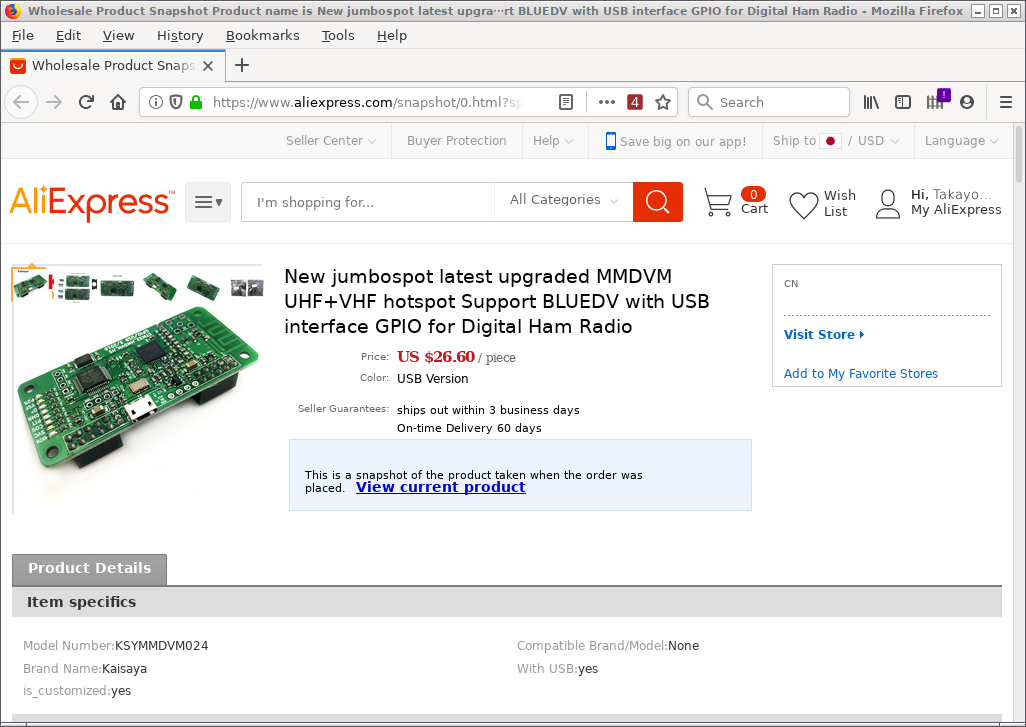
\includegraphics[width=15cm]{img/jumbospot-aliexpress.png}
 \caption{AliExpress で売られている JumboSPOT の例}
\end{figure}
この店では JumboSPOT に書き込まれているファームウエアの GPIO/USB 対応を選ぶことができたのですが、他所で売られているものについては分かりません。最悪の場合、ST-Link ケーブルや Raspberry Pi などを用意して、ファームウェアを書き換えることも想定する必要があります\footnote{GPIO 対応のファームウェアのまま、USB-UART アダプタ経由で繋ぐ方法については後述します。}。

なお、eBay や AliExpress で JumboSPOT を探すのは少し面倒で、「jumbospot」で見つからない場合は「MMDVM hotspot」などのキーワードでそれっぽい画像のものを探してみてください。

\section{免許申請について}

現時点において、JumboSPOT と DMR 機それぞれに対して無線局の免許を受けないと違法運用となってしまいます (これは、通信の相手方には自局が含まれないという法解釈によるものです)。既に開設済みの、移動する局の無線局免許に対して変更申請を行って TYT MD-380 のような DMR 機を増設することになるでしょうから、もう一方の JumboSPOT に対してはどうするかという話になります。選択肢はこうでしょうか。
\begin{enumerate}
 \item 既に開設済みの移動する局と同じコールサインを持つ、移動しない局としてホットスポットを開局する
 \item 誰かの名義を借りて、社団局としてホットスポットを開局する
 \item その他 (別個の無線局として免許を受けられれば何でも良いです)
\end{enumerate}
最近はホットスポット目的の移動しない局の開設は難しいという噂 \footnote{\url{http://www.bwt.jp/wiki/index.php?nora_gw}}もあるようなのですが、筆者は 2019 年 6 月上旬に 1. の方法で免許を受けました。ただし、移動しない局は JumboSPOT と ICOM IC-7200M (50W) で開局しているので、純粋に JumboSPOT のみで移動しない局を開局できるかどうかは分かりません。

工事設計書に記載する事項は、以下のようになります (電子申請 Lite 向けです)。
\begin{description}[style=nextline]
 \item[発射可能な電波の形式及び周波数の範囲] F7W 430MHz 
 \item[変調方式] F7W GMSK,四値周波数偏移変調 
 \item[終段管 (名称×個数・電圧)] ADF7021 × 1 個 3.3V 
 \item[定格出力] 20mW
\end{description}   
JumboSPOT の定格出力は 20mW ですが、希望する空中線電力は 1W と記載します。また、希望する電波の型式は (F7W しか使用しませんが) 4VA としてください。うっかり F7W と書いてしまうと、差し戻されます。既に開設済みの移動する局と同じコールサインを持つ移動しない局を開局する場合、移動する局のコールサインを申請書に記載する必要があります。移動しない局では空中線の形式も記載する必要がありますので、注意してください。

TYT MD-380 の時と異なり、変調方式に GMSK が含まれています。これは将来的に D-STAR への対応を行いたくなったときにすぐ運用できるよう記述しています。以下に送信機系統図の一例を示しますが、送信機系統図には DMR 以外のデジタル方式 (D-STAR, C4FM, NXDN, P25) も記しておくと良いでしょう。

\begin{figure}[H]
 \centering
 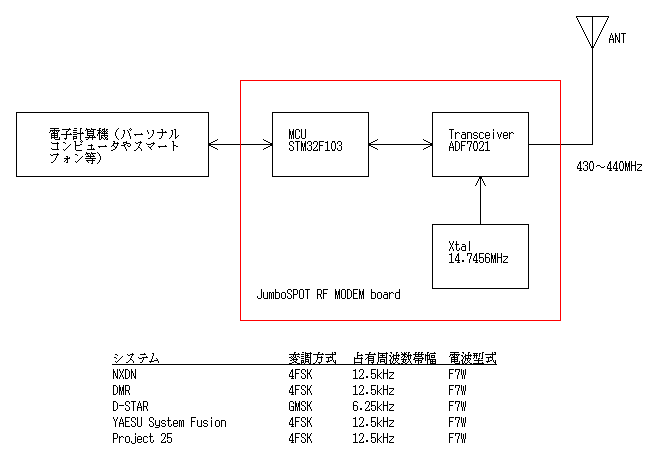
\includegraphics[width=15cm]{img/mmdvm-nopocsag.png}
 \caption{送信機系統図の例 (JumboSPOT)}
\end{figure}

MD-380 のときもそうでしたが、デジタル方式に対応する諸元は変調方式・占有周波数帯幅・電波型式だけ書いてあれば良く、これ以外については書かなくても良いようです (この辺りは相手も「分かっている」のかもしれません)\footnote{JumboSPOT はこの他に POCSAG 形式のページャ (かつてポケットベルと呼ばれた無線呼び出し) にも対応していますが、この申請を行う際は変調方式・占有周波数帯幅・電波型式に加え、通信速度・符号構成・誤り訂正符号を諸元に書く必要がありました。}。

\chapter{ホットスポットを作ろう}

\section{どう作るのか}

一般的には JumboSPOT ボードと同時に Raspberry Pi を購入し、Pi-Star を組み上げることが多いですが、ちょっと DMR の世界を覗いてみるにはお金がかかります (Raspberry Pi は手元にあれば何かと遊べますが、それでもあまりお安くありません)。今回は Raspberry Pi の代わりにパソコンを使用し、この上で MMDVMHost という制御プログラムを動作させることでホットスポットを作ってしまいます。

\section{用意するもの}

MMDVMHost は Linux 向けに書かれたプログラムなので Linux の動作するコンピュータが必要になる (そのために Raspberry Pi を用意する) のですが、ここでは VMware Player を使用した仮想 Linux マシンを用意します\footnote{VMware Player ではなく、使わなくなった Windows マシンに Linux をインストールしても良いでしょう。}。

まずは VMware Player を \url{https://www.vmware.com/go/downloadplayerpro-jp} からダウンロードし、インストールしておきます。次に OS インストールのための ISO イメージをダウンロードします。ここでは Raspberry Pi Desktop (Debian Buster with Raspberry Pi Desktop) を \url{https://www.raspberrypi.org/downloads/raspberry-pi-desktop/} からダウンロードし\footnote{ファイルサイズが 3GB 近くありますので、覚悟してください。}、インストールする場合で説明を行いますが、他に好きな Debian 系のものがあればそれを選んで構いません\footnote{Linux でなくとも、OpenBSD でも構いません。実際、筆者は OpenBSD-6.6/amd64 上で MMDVMHost を動かしています。}。

\section{仮想 Linux マシンの構築}

VMWare Player を起動し、ホームの「新規仮想マシンの作成(N)」から新規仮想マシン作成ウィザードを実行して、以下の操作を行います。仮想ディスクやメモリのサイズについてはとりあえず動かすための値なので、必要に応じて調整してください。

\begin{itemize}
 \item インストーラディスクイメージファイル (iso): 2021-01-11-raspios-buster-i386.iso
 \item ゲスト OS: Linux, バージョン: Debian 10.x
 \item 仮想マシン名: Linux-MMDVMHost
 \item ディスク最大サイズ: 40.0GB, 仮想ディスクを単一ファイルとして格納
 \item 「ハードウェアをカスタマイズ(C)」から、以下の設定を変更/確認し、「完了」
 \begin{itemize}
  \item メモリ: 2GB (2048MB)\footnote{デフォルトのままとしますが、ゲスト OS 推奨の最小メモリである 1GB (1024MB) に減らしても問題ありません。}
  \item ネットワークアダプタ: NAT
  \item USB コントローラ: あり
 \end{itemize}
\end{itemize}

OS のインストール時に余計なウィンドウが表示されると邪魔なので、一時的に環境設定を変更します。VMware Player 上部の「Player(P)」をクリックし、「ファイル(F)」→「環境設定(P)」をクリックします。「ソフトウェア アップデート」にある、「起動時に製品の更新を確認する(H)」と「必要に応じてソフトウェア コンポーネントを確認する(K)」のチェックを外しておいてください (OS のインストールが終わった後は、このチェックを付けておくことを忘れないように)。

これで、仮想マシンに OS をインストールする準備ができました。VMware Player が起動した状態で Linux-MMDVMHost を選択し、「仮想マシンの再生(L)」をクリックすると仮想マシンが起動します。起動後にメニューが表示されますが、操作を行えるようにするために\textbf{VMware Player のウィンドウ内を一度クリックしてから}以下の操作を行ってください。

\begin{itemize}
 \item Debian GNU/Linux menu (BIOS mode)
 \begin{itemize}
  \item カーソルキーで Graphical install を選択して Enter キーを押す (放っておくと Run with persistence となるので注意\footnote{Run with persistence で起動した場合は、起動後の Welcome to Raspberry Pi のメニューから Cancel を選択し、左上のラズベリーアイコンから Shutdown → Reboot で再起動してやり直します。})
 \end{itemize}
 \item Configure the keyboard
 \begin{itemize}
  \item Keymap to use: 日本語 106/109 キーボードの場合は Japanese、他のキーボードの場合は適切なものを選択
 \end{itemize}
 \item Partition disks
 \begin{itemize}
  \item Paratitioning method: Guided - use entire disk
  \item Select disk to partition: SCSI3 (0,0,0) (sda)
  \item Partitioning scheme: All files in one partition (recommended for new users)
  \item Finish partitioning and write changes to disk
  \item Write the changes to disks? の問いに Yes を選択
 \end{itemize}
 \item Install the system 〜 Configure the package manager
 \begin{itemize}
  \item 時間がかかり、画面がブラックアウトした場合はマウスを動かすか、 Shift や Ctrl 等動作に影響のないキーを押す
 \end{itemize}
 \item Install the GRUB boot loader on a hard disk
 \begin{itemize}
  \item Install the GRUB boot loader to the master boot record? の問いに Yes を選択
  \item Device for boot loader intallation: /dev/sda
 \end{itemize}
\end{itemize}

Finish the installation で Installation complete と表示された状態で Continue を選択すると、自動的に再起動します。再起動後は Welcome to Raspberry Pi のウィンドウが表示されますので Next をクリックし、以下の設定を行います。

\begin{itemize}
 \item Set Country
  \begin{itemize}
   \item Country: Japan
   \item Language: Japanese
   \item Timezone: Tokyo
   \item Use English Language にチェックが無いことを確認
   \item 日本語 106/109 キーボードの場合は Use US keyboard のチェックを外す
  \end{itemize}
  \item Change Password
  \begin{itemize}
   \item Enter New password, Confirm new password 共に同一のパスワードを入力\footnote{ユーザ名を入力する場面がありませんが、これは \tt{pi} が設定されています。}
  \end{itemize}
  \item Update Software: ここは Skip する
%  \item Error installing languages (The following packages have unmet dependencies) は OK を押してスキップ
% fcitx-frontend-qt4, fcitx-ui-classic, fcitx-module-x11, fcitx-frontend-gtk2, fcitx-frontend-gtk3, fcitx-mozc, fcitx-bin, fcitx-modules, tegaki-zinnia-japanese, mozc-utils-gui, fcitx
  \item Setup Complete: Done をクリック
\end{itemize}

言語設定を変更しているので、ここで必ず再起動します。左上のラズベリーのアイコンから Shutdown を選択し、Shutdown options の Reboot を選んで再起動してください。

再起動後に、設定の仕上げを行います。画面上端の $>$\_ と描かれたアイコンを押し、ターミナル (LXTerminal) を起動して以下のコマンドを入力してください\footnote{Raspberry Pi Desktop はインストール後すぐにプログラミングを開始できるよう、かなりの設定が済んでいる状態となっています。これ以外の Debian 系 Linux をインストールした場合は上記に加え、\tt{adduser ユーザ名 dialout} や \tt{apt-get install build-essential git} を行う必要もあります。} (コマンドの前の \verb+#+ や \verb+$+ はプロンプトなのでこれは入力しないように)。

\begin{verbatim}
$ sudo -i
# apt-get update
# apt-get upgrade
\end{verbatim}
\begin{itemize}
 \renewcommand{\labelitemi}{$\triangleright$}
 \item 続行しますか? [Y/n] の問いには \verb+y+
 \item (終了するには q を押して下さい) が表示された場合は \verb+q+
 \item 「The desktop has been updated.」が表示された場合は「OK」
\end{itemize}
\begin{verbatim}
# apt-get install fcitx-mozc
\end{verbatim}
\begin{itemize}
 \renewcommand{\labelitemi}{$\triangleright$}
 \item 続行しますか? [Y/n] の問いには \verb+y+
\end{itemize}

仮想マシンの用意はこれで完了です\footnote{\tt{apt-get install fcitx-mozc} により、日本語入力ができるようになっています。入力の切り替えは全角/半角キーもしくは Ctrl+Space で行いますが、Emacs を使用する場合は \tt{fcitx-config-gtk3} を使用し、「全体の設定」タブにある「入力メソッドのオンオフ」で Ctrl+Space を Shift+Space に変更しておくと良いでしょう。}。

\section{仮想マシンを終了させるには}
少し休憩してから、次のステップに進みましょう。

左上のラズベリーアイコンをクリックし、メニューからログアウトを選択して Shutdown options を表示させ、Shutdown で仮想マシンを終了させてください。もしくは、以下のコマンドで終了させることもできます。

\begin{verbatim}
$ sudo halt -p
\end{verbatim}

\section{MMDVMHost のコンパイル}

VMware Player を起動し、仮想マシン Linux-MMDVMHost が選択されている状態で「仮想マシンの再生」を行い、Raspberry Pi Desktop を起動します。

起動後、MMDVMHost のダウンロード・コンパイルを行います。画面上端の $>$\_ と描かれたアイコンを押してターミナル (LXTerminal) を起動し、以下のコマンドを入力してください\footnote{Raspberry Pi desktop ではこれだけで問題なく終わることを確認しています。これ以外の Debian 系 Linux でエラーが起こった場合は、\tt{sudo apt-get install build-essential}を実行してから再度試してみてください。}。

\begin{verbatim}
$ cd ~
$ git clone https://github.com/g4klx/MMDVMHost.git
$ cd MMDVMHost
$ make
\end{verbatim}

\chapter{ホットスポットを BrandMeister に繋いでみよう}

\section{BrandMeister アカウントを取得する}
アカウントを持たなくても BrandMeister ネットワークへの接続は可能ですが、ホットスポットに対する設定を行えるようにするため、最初に BrandMeister のアカウントを取得します。

\url{https://brandmeister.network/?page=register} へアクセスし、画面に表示された質問 (コールサイン・メールアドレス・パスワード等の項目) を埋めればアカウントの取得ができますが、申請してから実際に取得できるまでに時間がかかるため、この作業は最初に行っておくのが良いでしょう。Account Type は Personal User Account を選択してください。

\section{ホットスポットのパスワードを設定する}

ホットスポット上で動作する MMDVMHost が BrandMeister ネットワークへ接続する際、かつては Master (サーバ) 毎に設定される passw0rd 等のデフォルトのパスワードのままで問題ないとされていたのですが、2020 年 4 月頃からパスワードを設定することが推奨されています。BrandMeister アカウントを取得した後、SelfCare Settings (\url{https://brandmeister.network/?page=selfcare}) へアクセスし、以下の操作を行ってください。
\begin{itemize}
 \item HotSpot Security を On
 \item Password にパスワードを記述
 \item Save を押して保存
\end{itemize}
なお、このパスワードは Master 間で共通のものとなります。

\section{JumboSPOT の接続を確認する}

仮想 Linux マシンの動作するウィンドウがアクティブな状態で JumboSPOT ボードを USB に接続すると、「新しい USB デバイスが検出されました」というウィンドウが表示されます。仮想マシン名が Linux-MMDVMHost となっていることを確認し、「仮想マシンに接続」することで仮想 Linux マシンから JumboSPOT ボードを制御できるようになります。

もしこのウィンドウが表示されない場合は、VMWare Player の上部右側にデバイスの接続ステータスを示すアイコンが表示されていますので、右クリックして「接続 (ホストから切断)」してください。
仮想 Linux マシンの Terminal から以下のコマンドを実行し、JumboSPOT ボードが認識されていることを確認してください。

\begin{verbatim}
$ ls -l /dev/ttyACM*
crw-rw---- 1 root dialout 166, 0 Jul 16 16:43 /dev/ttyACM0
\end{verbatim}

以下のようになった場合は、JumboSPOT ボードの結線 (実際の配線及び仮想マシンへの接続) を確認してください。

\begin{verbatim}
$ ls -l /dev/ttyACM*
ls: cannot access '/dev/ttyACM*': No such file or directory
\end{verbatim}

ここからは、JumboSPOT は \verb+/dev/ttyACM0+ に接続されていることを前提に話を進めます。他のポートに接続されている場合は適宜読み替えてください。

\section{MMDVM.ini を設定する}

MMDVMHost を実行するためには設定ファイルである MMDVM.ini を適当なエディタ (nano, vi, Emacs 等) で編集する必要があります。これは、MMDVMHost をコンパイルしたディレクトリ (\verb+~/MMDVMHost+) の中にあります。以下にダウンロードした (オリジナルの) 状態からの変更点を示しますが、基本的に
\begin{itemize}
 \item 最低限必要な項目は設定する
 \item 使わないモード (DMR 以外) については全て無効化する
\end{itemize}
という考えに基づいて設定しています。

\begin{verbatim}
--------------------------------------------------------
[General]
Callsign=G9BF
Id=123456
\end{verbatim}
\begin{itemize}
 \renewcommand{\labelitemi}{$\triangleright$}
 \item \verb+Callsign+ にコールサインを、\verb+Id+ に DMR ID を設定します
\end{itemize}
\begin{verbatim}
Timeout=180
Duplex=1
\end{verbatim}
\begin{itemize}
 \renewcommand{\labelitemi}{$\triangleright$}
 \item JumboSPOT は Duplex 非対応のため、\verb+Duplex=0+ とします
\end{itemize}
\begin{verbatim}
# ModeHang=10
RFModeHang=10
NetModeHang=3
Display=None
Daemon=0

[Info]
RXFrequency=435000000
TXFrequency=435000000
\end{verbatim}
\begin{itemize}
 \renewcommand{\labelitemi}{$\triangleright$}
 \item \verb+RxFrequency+ と \verb+TxFrequency+ に使用する周波数 (Hz) を設定します
\end{itemize}
\begin{verbatim}
Power=1
# The following lines are only needed if a direct connection to a DMR master is being used
Latitude=0.0
Longitude=0.0
Height=0
Location=Nowhere
Description=Multi-Mode Repeater
URL=www.google.co.uk
\end{verbatim}
\begin{itemize}
 \renewcommand{\labelitemi}{$\triangleright$}
 \item \verb+Latitude+ 〜 \verb+URL+ の項目は適宜設定します
\end{itemize}
\begin{verbatim}

[Log]
# Logging levels, 0=No logging
DisplayLevel=1
FileLevel=1
FilePath=.
FileRoot=MMDVM
FileRotate=1

[CW Id]
Enable=1
\end{verbatim}
\begin{itemize}
 \renewcommand{\labelitemi}{$\triangleright$}
 \item CW ID は使用しないので必ず \verb+Enable=0+ にしてください
\end{itemize}
\begin{verbatim}
Time=10
# Callsign=

[DMR Id Lookup]
File=DMRIds.dat
Time=24

[NXDN Id Lookup]
File=NXDN.csv
Time=24

[Modem]
# Port=/dev/ttyACM0
# Port=/dev/ttyAMA0
Port=\\.\COM4
\end{verbatim}
\begin{itemize}
 \renewcommand{\labelitemi}{$\triangleright$}
 \item JumboSPOT を接続したポート \verb+Port=/dev/ttyACM0+ とします
 \item \verb+#+ の後は無視されます (コメントとして扱われます)
\end{itemize}
\begin{verbatim}
Protocol=uart
# Address=0x22
TXInvert=1
RXInvert=0
PTTInvert=0
TXDelay=100
RXOffset=0
TXOffset=0
\end{verbatim}
\begin{itemize}
 \renewcommand{\labelitemi}{$\triangleright$}
 \item \verb+RxOffset+ と \verb+TxOffset+ は JumboSPOT 裏面に書かれた値を設定します
\end{itemize}
\begin{verbatim}
DMRDelay=0
RXLevel=50
TXLevel=50
RXDCOffset=0
TXDCOffset=0
RFLevel=100
# CWIdTXLevel=50
# D-StarTXLevel=50
# DMRTXLevel=50
# YSFTXLevel=50
# P25TXLevel=50
# NXDNTXLevel=50
# POCSAGTXLevel=50
# FMTXLevel=50
RSSIMappingFile=RSSI.dat
UseCOSAsLockout=0
Trace=0
Debug=0

[Transparent Data]
Enable=0
RemoteAddress=127.0.0.1
RemotePort=40094
LocalPort=40095
# SendFrameType=0

[UMP]
Enable=0
# Port=\\.\COM4
Port=/dev/ttyACM1

[D-Star]
Enable=1
\end{verbatim}
\begin{itemize}
 \renewcommand{\labelitemi}{$\triangleright$}
 \item D-STAR は使用しないので \verb+Enable=0+ とします
\end{itemize}
\begin{verbatim}
Module=C
SelfOnly=0
AckReply=1
AckTime=750
AckMessage=0
ErrorReply=1
RemoteGateway=0
# ModeHang=10
WhiteList=

[DMR]
Enable=1
Beacons=0
BeaconInterval=60
BeaconDuration=3
ColorCode=1
\end{verbatim}
\begin{itemize}
 \renewcommand{\labelitemi}{$\triangleright$}
 \item 無線機に設定する Color Code となるので、この値は確認しておいてください
\end{itemize}
\begin{verbatim}
SelfOnly=0
EmbeddedLCOnly=0
DumpTAData=1
# Prefixes=234,235
# Slot1TGWhiteList=
# Slot2TGWhiteList=
CallHang=3
TXHang=4
# ModeHang=10
# OVCM Values, 0=off, 1=rx_on, 2=tx_on, 3=both_on, 4=force off
# OVCM=0

[System Fusion]
Enable=1
\end{verbatim}
\begin{itemize}
 \renewcommand{\labelitemi}{$\triangleright$}
 \item System Fusion (C4FM) は使用しないので \verb+Enable=0+ とします
\end{itemize}
\begin{verbatim}
LowDeviation=0
SelfOnly=0
TXHang=4
RemoteGateway=0
# ModeHang=10

[P25]
Enable=1
\end{verbatim}
\begin{itemize}
 \renewcommand{\labelitemi}{$\triangleright$}
 \item P25 は使用しないので \verb+Enable=0+ とします
\end{itemize}
\begin{verbatim}
NAC=293
SelfOnly=0
OverrideUIDCheck=0
RemoteGateway=0
TXHang=5
# ModeHang=10

[NXDN]
Enable=1
\end{verbatim}
\begin{itemize}
 \renewcommand{\labelitemi}{$\triangleright$}
 \item NXDN は使用しないので \verb+Enable=0+ とします
\end{itemize}
\begin{verbatim}
RAN=1
SelfOnly=0
RemoteGateway=0
TXHang=5
# ModeHang=10

[POCSAG]
Enable=1
\end{verbatim}
\begin{itemize}
 \renewcommand{\labelitemi}{$\triangleright$}
 \item POCSAG は使用しないので \verb+Enable=0+ とします
\end{itemize}
\begin{verbatim}
Frequency=439987500

[FM]
Enable=1
\end{verbatim}
\begin{itemize}
 \renewcommand{\labelitemi}{$\triangleright$}
 \item FM は使用しないので \verb+Enable=0+ とします
\end{itemize}
\begin{verbatim}
# Callsign=G4KLX
CallsignSpeed=20
CallsignFrequency=1000
CallsignTime=10
CallsignHoldoff=0
CallsignHighLevel=50
CallsignLowLevel=20
CallsignAtStart=1
CallsignAtEnd=1
CallsignAtLatch=0
RFAck=K
ExtAck=N
AckSpeed=20
AckFrequency=1750
AckMinTime=4
AckDelay=1000
AckLevel=50
# Timeout=180
TimeoutLevel=80
CTCSSFrequency=88.4
CTCSSThreshold=30
# CTCSSHighThreshold=30
# CTCSSLowThreshold=20
CTCSSLevel=20
KerchunkTime=0
HangTime=7
AccessMode=1
COSInvert=0
RFAudioBoost=1
MaxDevLevel=90
ExtAudioBoost=1

[D-Star Network]
Enable=1
\end{verbatim}
\begin{itemize}
 \renewcommand{\labelitemi}{$\triangleright$}
 \item D-STAR は使用しないので \verb+Enable=0+ とします
\end{itemize}
\begin{verbatim}
GatewayAddress=127.0.0.1
GatewayPort=20010
LocalPort=20011
# ModeHang=3
Debug=0

[DMR Network]
Enable=1
# Type may be either 'Direct' or 'Gateway'. When Direct you must provide the Master's
# address as well as the Password, and for DMR+, Options also.
Type=Gateway
\end{verbatim}
\begin{itemize}
 \renewcommand{\labelitemi}{$\triangleright$}
 \item DMRGateway を使用しないので \verb+Type=Direct+ とします (省略した場合、\verb+Type=Gateway+ と同義です)
\end{itemize}
\begin{verbatim}
Address=127.0.0.1
Port=62031
Local=62032
# Password=P@ssw0rd1234
\end{verbatim}
\begin{itemize}
 \renewcommand{\labelitemi}{$\triangleright$}
 \item ここでは US Master (3101) \verb+Address=107.191.99.14 Password=+(BrandMeister の HotSport Security で設定したパスワード) を指定します\footnote{Master の IP アドレスは、DMR\_Hosts.txt (\url{http://www.pistar.uk/downloads/DMR_Hosts.txt}) を参照してください。日本向けの TalkGroup はかつて存在した Japan Master でしか使えないという情報がありましたが、これは全くの誤りで、どこの Master に接続しても同等のサービスを受けることができます。}
\end{itemize}
\begin{verbatim}
Jitter=360
Slot1=1
Slot2=1
# Options=
# ModeHang=3
Debug=0

[System Fusion Network]
Enable=1
\end{verbatim}
\begin{itemize}
 \renewcommand{\labelitemi}{$\triangleright$}
 \item System Fusion (C4FM) は使用しないので \verb+Enable=0+ とします
\end{itemize}
\begin{verbatim}
LocalAddress=127.0.0.1
LocalPort=3200
GatewayAddress=127.0.0.1
GatewayPort=4200
# ModeHang=3
Debug=0

[P25 Network]
Enable=1
\end{verbatim}
\begin{itemize}
 \renewcommand{\labelitemi}{$\triangleright$}
 \item P25 は使用しないので \verb+Enable=0+ とします
\end{itemize}
\begin{verbatim}
GatewayAddress=127.0.0.1
GatewayPort=42020
LocalPort=32010
# ModeHang=3
Debug=0

[NXDN Network]
Enable=1
\end{verbatim}
\begin{itemize}
 \renewcommand{\labelitemi}{$\triangleright$}
 \item NXDN は使用しないので \verb+Enable=0+ とします
\end{itemize}
\begin{verbatim}
Protocol=Icom
LocalAddress=127.0.0.1
LocalPort=14021
GatewayAddress=127.0.0.1
GatewayPort=14020
# ModeHang=3
Debug=0

[POCSAG Network]
Enable=1
\end{verbatim}
\begin{itemize}
 \renewcommand{\labelitemi}{$\triangleright$}
 \item POCSAG は使用しないので \verb+Enable=0+ とします
\end{itemize}
\begin{verbatim}
LocalAddress=127.0.0.1
LocalPort=3800
GatewayAddress=127.0.0.1
GatewayPort=4800
# ModeHang=3
Debug=0

[TFT Serial]
# Port=modem
Port=/dev/ttyAMA0
Brightness=50

[HD44780]
Rows=2
Columns=16

# For basic HD44780 displays (4-bit connection)
# rs, strb, d0, d1, d2, d3
Pins=11,10,0,1,2,3

# Device address for I2C
I2CAddress=0x20

# PWM backlight
PWM=0
PWMPin=21
PWMBright=100
PWMDim=16

DisplayClock=1
UTC=0

[Nextion]
# Port=modem
Port=/dev/ttyAMA0
Brightness=50
DisplayClock=1
UTC=0
#Screen Layout: 0=G4KLX 2=ON7LDS
ScreenLayout=2
IdleBrightness=20

[OLED]
Type=3
Brightness=0
Invert=0
Scroll=1
Rotate=0
Cast=0
LogoScreensaver=1

[LCDproc]
Address=localhost
Port=13666
#LocalPort=13667
DimOnIdle=0
DisplayClock=1
UTC=0

[Lock File]
Enable=0
File=/tmp/MMDVM_Active.lck

[Remote Control]
Enable=0
\end{verbatim}
\begin{itemize}
 \renewcommand{\labelitemi}{$\triangleright$}
 \item 外部からの攻撃を受けないよう、\verb+Enable=0+ であることを確認してください
\end{itemize}
\begin{verbatim}
Port=7642
--------------------------------------------------------
\end{verbatim}

\section{MMDVMHost を起動する}

MMDVM.ini の設定が終わったので、MMDVMHost を起動して実際に BrandMeister に接続します。

\begin{verbatim}
$ cd ~/MMDVMHost
$ ./MMDVMHost ./MMDVM.ini
\end{verbatim}

MMDVMHost は引数を指定しない場合、\verb+/etc/MMDVM.ini+ を参照します。しかしここでは \verb+~/MMDVMHost+ にある MMDVM.ini を使用するよう引数を指定しています。特に問題が無ければ、以下のようなメッセージが表示されるはずです。

\begin{verbatim}
--------------------------------------------------------
$ ./MMDVMHost ./MMDVM.ini
I: 2020-12-13 01:40:43.080 This software is for use on amateur radio 
networks only,
I: 2020-12-13 01:40:43.080 it is to be used for educational purposes 
only. Its use on
I: 2020-12-13 01:40:43.080 commercial networks is strictly prohibited.
I: 2020-12-13 01:40:43.080 Copyright(C) 2015-2020 by Jonathan Naylor,
 G4KLX and others
M: 2020-12-13 01:40:43.080 MMDVMHost-20201209 is starting
M: 2020-12-13 01:40:43.080 Built 10:29:40 Dec 13 2020 (GitID #6e05225)
I: 2020-12-13 01:40:43.080 General Parameters
I: 2020-12-13 01:40:43.080     Callsign: XXXXXX
I: 2020-12-13 01:40:43.080     Id: XXXXXXX
I: 2020-12-13 01:40:43.080     Duplex: no
I: 2020-12-13 01:40:43.080     Timeout: 180s
I: 2020-12-13 01:40:43.080     D-Star: disabled
I: 2020-12-13 01:40:43.080     DMR: enabled
I: 2020-12-13 01:40:43.080     YSF: disabled
I: 2020-12-13 01:40:43.080     P25: disabled
I: 2020-12-13 01:40:43.080     NXDN: disabled
I: 2020-12-13 01:40:43.080     POCSAG: enabled
I: 2020-12-13 01:40:43.080     FM: disabled
I: 2020-12-13 01:40:43.080 Modem Parameters
I: 2020-12-13 01:40:43.080     Port: /dev/ttyACM0
I: 2020-12-13 01:40:43.080     Protocol: uart
I: 2020-12-13 01:40:43.080     RX Invert: no
I: 2020-12-13 01:40:43.080     TX Invert: yes
I: 2020-12-13 01:40:43.080     PTT Invert: no
I: 2020-12-13 01:40:43.080     TX Delay: 100ms
I: 2020-12-13 01:40:43.080     RX Offset: 1100Hz
I: 2020-12-13 01:40:43.080     TX Offset: 1100Hz
I: 2020-12-13 01:40:43.080     RX DC Offset: 0
I: 2020-12-13 01:40:43.080     TX DC Offset: 0
I: 2020-12-13 01:40:43.080     RF Level: 100.0%
I: 2020-12-13 01:40:43.080     DMR Delay: 0 (0.0ms)
I: 2020-12-13 01:40:43.080     RX Level: 50.0%
I: 2020-12-13 01:40:43.080     CW Id TX Level: 50.0%
I: 2020-12-13 01:40:43.080     D-Star TX Level: 50.0%
I: 2020-12-13 01:40:43.080     DMR TX Level: 50.0%
I: 2020-12-13 01:40:43.080     YSF TX Level: 50.0%
I: 2020-12-13 01:40:43.080     P25 TX Level: 50.0%
I: 2020-12-13 01:40:43.080     NXDN TX Level: 50.0%
I: 2020-12-13 01:40:43.080     POCSAG TX Level: 50.0%
I: 2020-12-13 01:40:43.080     FM TX Level: 50.0%
I: 2020-12-13 01:40:43.080     TX Frequency: XXXXX0000Hz (XXXXX1100Hz)
I: 2020-12-13 01:40:43.080     Use COS as Lockout: no
M: 2020-12-13 01:40:43.081 Opening the MMDVM
I: 2020-12-13 01:40:45.130 MMDVM protocol version: 1, description: MM
DVM_HS_Hat-v1.5.1b 20191201 14.7456MHz ADF7021 FW by CA6JAU GitID #ec
4fd74
I: 2020-12-13 01:40:45.170 Display Parameters
I: 2020-12-13 01:40:45.170     Type: None
I: 2020-12-13 01:40:45.170 No valid display found, disabling
I: 2020-12-13 01:40:45.540 DMR Network Parameters
I: 2020-12-13 01:40:45.540     Type: Direct
I: 2020-12-13 01:40:45.540     Address: 107.191.99.14
I: 2020-12-13 01:40:45.540     Port: 62031
I: 2020-12-13 01:40:45.540     Local: 62032
I: 2020-12-13 01:40:45.540     Jitter: 360ms
I: 2020-12-13 01:40:45.540     Slot 1: enabled
I: 2020-12-13 01:40:45.540     Slot 2: enabled
I: 2020-12-13 01:40:45.540     Mode Hang: 3s
I: 2020-12-13 01:40:45.541 Info Parameters
I: 2020-12-13 01:40:45.541     Callsign: XXXXXX
I: 2020-12-13 01:40:45.541     RX Frequency: XXXXX0000Hz
I: 2020-12-13 01:40:45.541     TX Frequency: XXXXX0000Hz
I: 2020-12-13 01:40:45.541     Power: 1W
I: 2020-12-13 01:40:45.541     Latitude: X.XXXXXXdeg N
I: 2020-12-13 01:40:45.541     Longitude: X.XXXXXXdeg E
I: 2020-12-13 01:40:45.541     Height: Xm
I: 2020-12-13 01:40:45.541     Location: "XXXXXXXXXXXXXX"
I: 2020-12-13 01:40:45.541     Description: "XXXXXXXXXXXXXXXXXXX"
I: 2020-12-13 01:40:45.541     URL: "XXXXXXXXXXXXXX"
M: 2020-12-13 01:40:45.541 Opening DMR Network
I: 2020-12-13 01:40:45.541 RSSI
I: 2020-12-13 01:40:45.541     Mapping File: RSSI.dat
I: 2020-12-13 01:40:45.541 Loaded 0 RSSI data mapping points from RSS
I.dat
I: 2020-12-13 01:40:45.541 DMR Id Lookups
I: 2020-12-13 01:40:45.541     File: DMRIds.dat
I: 2020-12-13 01:40:45.541     Reload: 24 hours
I: 2020-12-13 01:40:47.272 Loaded 180628 IDs to lookup table - DMRIds.dat
I: 2020-12-13 01:40:47.272 DMR RF Parameters
I: 2020-12-13 01:40:47.273 Started the DMR Id lookup reload thread
I: 2020-12-13 01:40:47.273     Id: XXXXXXX
I: 2020-12-13 01:40:47.273     Color Code: 1
I: 2020-12-13 01:40:47.273     Self Only: no
I: 2020-12-13 01:40:47.273     Embedded LC Only: no
I: 2020-12-13 01:40:47.273     Dump Talker Alias Data: yes
I: 2020-12-13 01:40:47.273     Prefixes: 0
I: 2020-12-13 01:40:47.273     Call Hang: 3s
I: 2020-12-13 01:40:47.273     TX Hang: 3s
I: 2020-12-13 01:40:47.273     Mode Hang: 10s
I: 2020-12-13 01:40:47.273     OVCM: off
I: 2020-12-13 01:40:47.273     DMR Roaming Beacons Type: off
M: 2020-12-13 01:40:47.273 MMDVMHost-20201209 is running
I: 2020-12-13 01:40:57.290 Opening UDP port on 62032
D: 2020-12-13 01:40:57.610 DMR, Sending authorisation
D: 2020-12-13 01:40:57.930 DMR, Sending configuration
M: 2020-12-13 01:40:58.250 DMR, Logged into the master successfully
--------------------------------------------------------
\end{verbatim}

もし \verb+/dev/ttyACM0+ がオープンできないといったエラーが発生した場合、\verb+/dev/ttyACM0+ がきちんと認識できているかどうか確認してください\footnote{Raspberry Pi Desktop では既に設定されていますが、これ以外の Linux では \tt{/dev/ttyACM0} を使用するユーザがグループ dialout に加わっているかを確認する必要もあるかもしれません。}。

BrandMeister ネットワークに接続できない場合、接続先の IP アドレスやパスワードが間違っていないか、MMDVM.ini の [DMR Network] セクションの Address や Password の設定を見直してください。もし BrandMeister Master にトラブルがあり接続できない場合は、他の Master を使用する設定を試してみてください。

\section{受信するトークグループを設定しよう}

トークグループには二種類あり、無線機の PTT ボタンを押して一時的に参加する Dynamic なもの (15 分程度で退出します) と、PTT を押さずとも参加状態となっている Static なものがあります。BrandMeister 側で設定を行わない場合は全て Dynamic 扱いとなっており、またトークグループを受信するためにはそのトークグループへ参加している必要があるために PTT を押さないと何も聞こえません (そして PTT を押すことでトークグループに参加していることがバレてしまう)。

BrandMeister のアカウントを取得することで Static トークグループの設定を行えるようになりますから、まずはこれを設定してみましょう。

ホットスポットを BrandMeister ネットワークに接続した後に BrandMeister の web page (\url{https://brandmeister.network/?page=login}) へアクセスし、ログインを行うと画面左側のメニューに「My hotspots」が増えています。ここに表示されたホットスポットの DMR ID をクリックしてください。

設定画面の下の方に「Static Talkgroups」という項目がありますので、受信を希望したいトークグループを設定します。日本における主なものとしては
\begin{itemize}
 \item 440110 国内非常通信/訓練
 \item 44120 国内ラグチュー (メイン)
 \item 44121 国内ラグチュー (サブ)
\end{itemize}
があり、全世界規模のものとしては
\begin{itemize}
 \item 91 World-Wide
\end{itemize}
があります。これ以外にどのようなトークグループがあるかについては \url{http://www.pistar.uk/downloads/TGList_BM.txt} や \url{http://www.mw0mwz.co.uk/dmr_bm_talkgroups.php} を見てください。

BrandMeister は Hoseline (\url{https://hose.brandmeister.network/}) にアクセスすると web ブラウザからトークグループの会話をワッチすることができますから、ここで雰囲気を掴んでから設定するのも良いでしょう。

\section{無線機を設定する}

MMDVMHost の設定は終わったので、今度は無線機の設定です。ここでは TYT MD-380 を例に説明しますが、基本的にはどの DMR 機でも対応できるはずです。

\subsection*{設定を始める前に}

DMR 機はプログラミングケーブルを使用して無線機とパソコンを繋ぎ、CPS (Customer Programming Software) と呼ばれるプログラムを起動して各種設定を行うのが特徴です。早速無線機の設定を行って運用を始めたいところですが、まず最初にすることは無線機からデータをダウンロードして保存することです。これは、最初にダウンロードしたデータを残しておかないと万一のときに初期状態へ戻せないという理由によるものです (無線機のボタン操作等で、リセットするような機能はありません)。

まっさらな状態のデータを保存したら、早速設定を始めます。

\subsection*{General Setting}

Radio ID に DMR ID を忘れずに設定してください。

\subsection*{Digital Contacts}

参加したい BrandMeister のトークグループを登録します。以下に一例を示します。

\begin{center}
 \begin{tabular}{|c|c|c|c|}
  \hline
  {Contact Name} & {Call Type} & {Call ID} & {Call Receive Tone} \\
  \hline
  {BM WorldWide} & {Group Call} & 91 & No \\
  {BM\_Japan Main} & {Group Call} & 44120 & No \\
  {BM\_Japan Sub} & {Group Call} & 44121 & No \\
  {BM\_Japan Emg} & {Group Call} & 440110 & No \\
  \hline
 \end{tabular}
\end{center}

\subsection*{Channels Information}

ここは設定項目が多いです。ウィンドウのスクリーンショットをまずはお見せします。

\begin{figure}[H]
 \begin{center}
  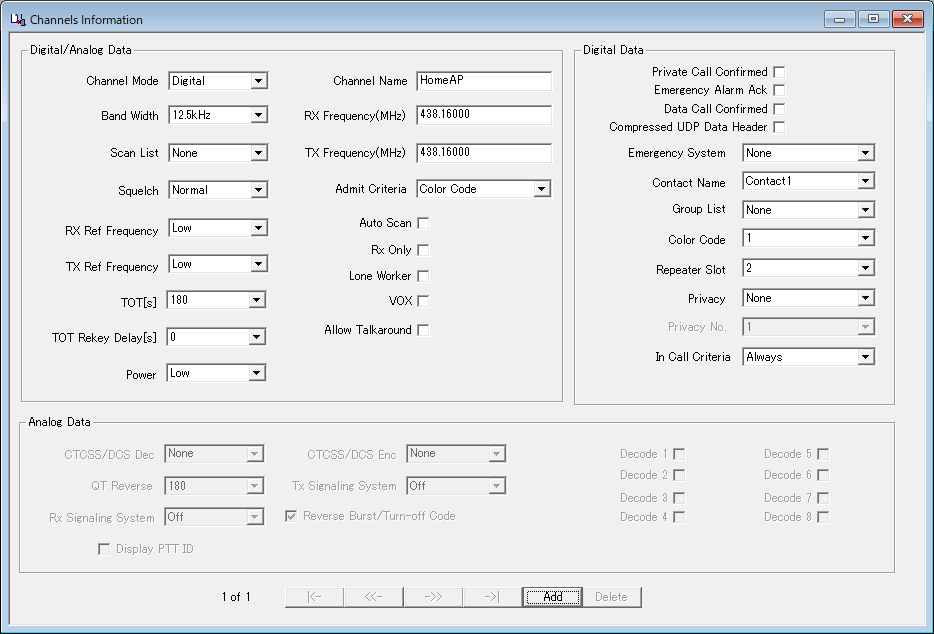
\includegraphics[width=15cm]{img/md380cps-channelinfo.png}
 \end{center}
 \caption{MD-380 CPS: Channels Information}
\end{figure}

\begin{itemize}
 \item Digital/Analog Data
 \begin{itemize} 
  \item Channel Mode: Digital
  \item Channel Name: HomeAP
  \begin{itemize}
   \renewcommand{\labelitemiii}{$\triangleright$}
   \item この名前は一例で、適当な分かりやすいものを付けると良いでしょう
  \end{itemize}
  \item Rx Frequency (MHz): MMDVM.ini の TxFrequency の値を MHz に直した値
  \item Tx Frequency (MHz): MMDVM.ini の RxFrequency の値を MHz に直した値
  \item Admit Criteria: Color Code
  \begin{itemize}
   \renewcommand{\labelitemiii}{$\triangleright$}
   \item Always だといつでも送信できてしまうので、同じ Color Code で誰かが送信している時は送信を禁止するようにします
  \end{itemize}
  \item TOT[s]: 180
  \begin{itemize}
   \renewcommand{\labelitemiii}{$\triangleright$}
   \item デフォルトの 60 は短いので、少しのばします
  \end{itemize}
  \item Power: Low
  \begin{itemize}
   \renewcommand{\labelitemiii}{$\triangleright$}
   \item ホットスポット相手に送信するので Power は Low で十分です
  \end{itemize}
 \end{itemize}
 \item Digital Data
 \begin{itemize}
  \item Contact Name: よく出入りするトークグループを選択
  \item Group List: None
  \begin{itemize}
   \renewcommand{\labelitemiii}{$\triangleright$}
   \item None とします (None 以外の設定を行う場合は、Digital RX Group Lists に受信したいトークグループのリストを作成しないと受信ができません)
  \end{itemize}
  \item Color Code: MMDVM.ini の ColorCode の値
  \item Repeater Slot: 2
  \begin{itemize}
   \renewcommand{\labelitemiii}{$\triangleright$}
   \item DMR において、レピーター/ホットスポット経由での通信は TimeSlot 2 を使います
  \end{itemize}
  \item Privacy: None
  \begin{itemize}
   \renewcommand{\labelitemiii}{$\triangleright$}
   \item None 以外の設定は禁止です (暗号化を使用してはいけません)
  \end{itemize}
 \end{itemize}
\end{itemize}

\subsection*{Zone Information}

Zone1 等の適当なゾーンに、先程作成した HomeAP のチャンネルを含めておきます。

\begin{figure}[H]
 \begin{center}
  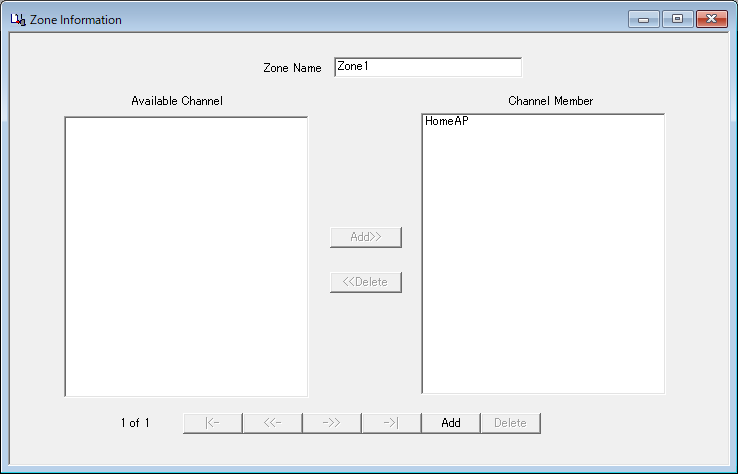
\includegraphics[width=11.9cm]{img/md380cps-zoneinfo.png}
 \end{center}
 \caption{MD-380 CPS: Zone Info}
\end{figure}

無線機ではゾーンとチャンネルを設定すると、これに伴う設定 (Digital Contacts など) も併せて行われます。ここではホットスポット相手に通信を行うことになりますので、Digital Contacts とこれに対応した Channels Information が増えていくような形になるでしょう\footnote{海外においては、よく使われるトークグループや著名なレピーター (BrandMeister へのアクセスポイントも兼ねています) の周波数をまとめた CodePlug と呼ばれる CPS 用のデータが流通しています。ホットスポットでの運用が主体となる日本においては、どうなるでしょうか。}。

ここまで設定することで、DMR 機から BrandMeister を経由して交信できるはずです。もしうまくいかない場合は、再度今までの作業内容を確認してみてください。

\begin{itemize}
 \item JumboSPOT の接続は問題ないか
 \item MMDVMHost は起動し、JumboSPOT を認識できているか
 \item MMDVMHost は BrandMeister サーバに接続できているか
 \item MMDVM.ini の設定は問題ないか (周波数・Offset・ColorCode など)
 \item 無線機の設定は問題ないか (周波数・Offset・ColorCode・TalkGroup など)
 \item BrandMeister の設定は問題ないか (Static Talkgroups)
\end{itemize}

\chapter{参考資料}

\section{日本語で書かれたもの}

以下に、筆者が DMR 機での開局・変更申請を行う際に参考にした日本語の情報源を示します (本文中で触れたページも含まれています)。

\begin{description}[style=nextline]
 \item[BM Japan (BrandMeister)] \url{https://wiki.brandmeister.network/index.php/Japan}
 \item[DMR (Digital Mobile Radio)/D-STAR REFLECTOR の構築 (JQ1BWT)] \url{http://www.bwt.jp/wiki/?DMR_Reflector}
 \item[MultiMode Digital Voice Modemで拓くアマチュア無線デジタル音声の新潮流 Kindle版 (JE4SMQ)] \url{https://www.amazon.co.jp/dp/B07MHD39KF}
 \item[TalkGroup/44130 フリートーク DMR 勉強会 (BrandMeister)] \url{https://wiki.brandmeister.network/index.php/TalkGroup/44130}
 \item[XRF リフレクター同好会 (JA1COU)] \url{https://ja1cou.wixsite.com/ja1cou/}
 \item[ラブラドール ななの部屋のブログ] \url{http://h7nana.cocolog-nifty.com/blog/cat24137161/}
\end{description}

\section{英語で書かれたもの}

DMR 自体の情報は海外の方が豊富であり、英語に抵抗が無ければこちらを参照した方が早いです。

\begin{description}[style=nextline]
 \item[Amateur Radio Guide to Digital Mobile Radio (DMR) (DMR-MARC)] \url{http://www.dmr-marc.net/media/Amateur_Radio_Guide_to_DMR_Rev_I_20150510.pdf}
 \item[Comparison of DMR radios (Radiosification)] \url{https://radiosification.blogspot.com/2017/11/comparison-of-dmr-radios.html}
 \item[DMR Info Site (K3NXU)] \url{https://www.miklor.com/DMR/}
 \item[Dynamic talkgroup and Static Talkgroup on Brandmeister (Ailunce)] \url{https://www.ailunce.com/blog/Dynamic-talkgroup-and-Static-Talkgroup-on-Brandmeister}
 \item[Homebrew/MMDVM (BrandMeister)] \url{https://wiki.brandmeister.network/index.php/Homebrew/MMDVM}
 \item[You and Your Tytera MD-380 DMR (Adafruit)] \url{https://learn.adafruit.com/tytera-md-380-dmr/programming}
\end{description}

参考とした多くの情報源、およびその作者に感謝します。

\chapter{おわりに}

DMR を取り巻く状況は日々変化しつつあり、本書の内容もすぐに古くなってしまう可能性は高いです。最新の情報はネット上で調べることをおすすめしますが、もし可能なら、後に続く人達のために「試したこと」「その結果うまくいったこと」「逆にうまくできなかったこと」をブログなどの (誰かが参照できる) 形で残してもらえると助かります。

本書が DMR を始める際の何らかの参考になれば、幸甚です。

\chapter{改訂履歴}
\begin{description}[style=nextline]
 \item[20190822] 初版
 \item[20200222] MMDVM.ini の設定例において、接続先を Japan Master (4401) から US Master (3101) に変更。
 \item[20200223] 仮想 Linux マシンに使用するディストリビューションを BunsenLabs Helium (Build2) から Debian Buster with Raspberry Pi Desktop (32bit) に変更。
 \item[20201213] 仮想 Linux マシンにおける日本語入力切り替えの方法、ホットスポットのパスワード設定に関する記述を追加。MMDVM.ini の説明および起動時のログを MMDVMHost-2019131→MMDVMHost-20201209 に合わせ変更。RadioID.net のスクリーンショット差し替え。
 \item[20210703] TYT MD-380 の販売状況について追記。URL と Raspberry Pi Desktop の ISO イメージファイル名および操作方法を 2021-01-11-raspios-buster-i386.iso に合わせて修正。VMware Player の操作方法は 16.x 向けに修正。MMVDM.ini の設定例を修正 (設定内容は変わらず)。
 \item[20220227] USB 非対応版 JumboSPOT を使用する場合の補足を追加。
\end{description}

\appendix
\chapter{Retevis RT80 を使えるようにするまで}

\section{何故 RT80 なのか}

TYT MD-380 は確かに DMR を始めるには良い無線機です。ですが、もう少し安い無線機があれば DMR への間口がもうちょっと広がるのではないかと思い、探してみたところ Retevis RT80 という無線機を見つけました。

\begin{figure}[H]
 \centering
 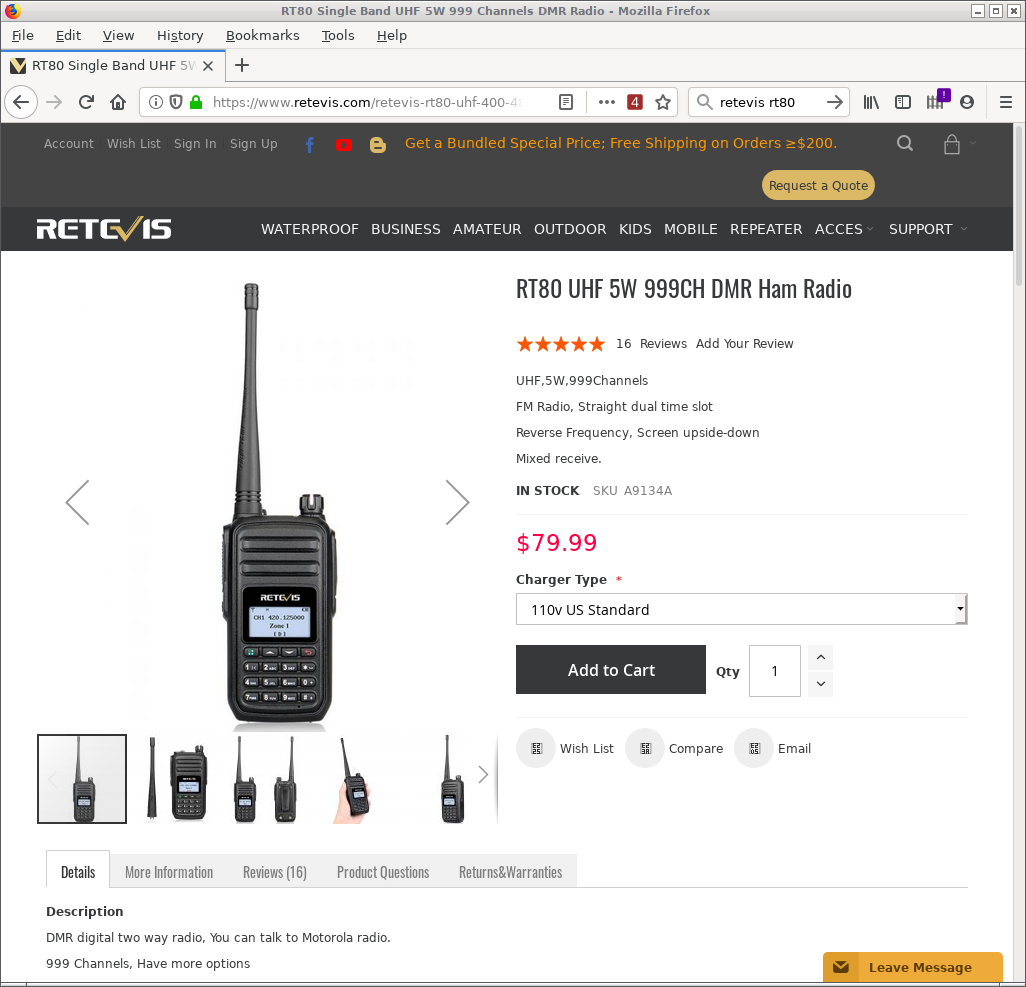
\includegraphics[width=15cm]{img/rt80-web.png}
 \caption{Retevis RT80}
\end{figure}

値段が安い\footnote{2018 年 10 月の時点での話です。}だけでなく、FM ラジオとしても使える (ただし受信範囲は 87.5 〜 108.0 MHz) という部分も魅力的です。
Retevis の商品販売ページ\footnote{かつては \url{https://www.retevis.com/retevis-rt80-uhf-400-480mhz-5w-999-channels-dmr-radio} に存在しましたが、2021 年 7 月時点ではディスコンとなってしまったのか、アクセスできなくなっています。}から早速発注しても良かったのですが、その前に少し調べてみることにしました。

\section{買う前にできること}

ありがたいことに、RT80 の CPS はサポートページ\footnote{かつては \url{https://www.retevis.com/resources-center} に存在したものの、2021 年 7 月時点では無線機のページからソフトウェアをダウンロードするように変わっており、無線機のページごと消滅した模様。}からダウンロード可能な状態になっています。無線機は手元になくとも、CPS の中には無線機を知るためのヒントが隠されているかもしれませんので試しにダウンロードしてインストールします。早速 CPS (RT80.exe) を秀丸エディタで開いてみると…

\begin{figure}[H]
 \centering
 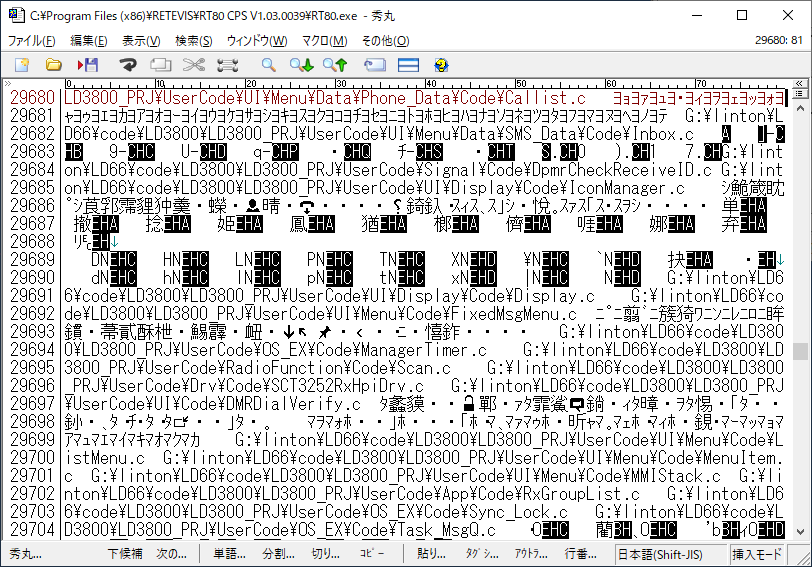
\includegraphics[width=15cm]{img/rt80-cps.png}
 \caption{RT80 CPS (RT80.exe) をテキストエディタで表示}
\end{figure}

linton, LD3800, SCT3252 というキーワードが出てきます。調べてみるに、RT80 は Linton LD-3800\footnote{扱いをやめたのか、\url{http://www.linton.cn/} から見つけることはできない。} の OEM らしく、他にも TID TD-DP580\footnote{\url{https://www.tid-china.com/index.php?m=product&a=details&content_id=24}} や TSSD TS-D8200R\footnote{\url{https://www.aliexpress.com/item/32862477160.html}} というメーカー・型番でも売られています。LD-3800 は FCC ID を持っており (2AN96DM18301)、FCC ID Search では回路図や送信機系統図は公開されていないものの Test Report からスプリアス発射強度の測定結果を、Int Photos から内部写真を見ることができます\footnote{\url{https://fccid.io/2AN96DM18301}}。内部写真には AT と書かれたチップが写っていることから、おそらく AT1846S の類が使われている可能性があると判断します。

また、FCC ID Search を探ると Kydera DM-6R\footnote{\url{https://fccid.io/VO6DM-6R}} という DMR 機や Quantun QP-990-U1\footnote{\url{https://fccid.io/XMHQP-990-U1}} という dPMR 機の情報も入手できます。こちらは回路図や送信機系統図も見ることができるので、役に立つかどうかは後で考えるとしてとりあえず押さえておきます。

SCT3252 は dPMR/DMR 向けのベースバンドプロセッサです\footnote{\url{http://www.sicommtech.com/en/products/sct3252.html}}。「SCT3252 schematic」で検索すると Kirisun FM540 (DMR機) のサービスマニュアルが見つかりますので\footnote{\url{http://doc.xdevs.com/doc/Misc/Kirisun/FM54-service-manual020160722.pdf}}、こちらも押さえておきます。

集まった情報から、
\begin{itemize}
 \item 値段も安いし仮に免許が下りなかったとしても FM ラジオとしては使える
 \item イマドキの無線機なので新スプリアス基準は満たしていそう
 \item SCT3252 と AT1846S 辺りのチップを使っていそう
 \item 部品点数は少なそうだしそんなに解析は難しくない…んじゃないかな?
\end{itemize}
と判断し、RT80 を発注することにしました。

\section{分解しないことには分からない}

Retevis の商品販売ページから RT80 を発注し、しばらくすれば\footnote{\url{海外通販なので、amazon.co.jp 辺りの時間感覚と同列に扱わないように。}}こんな感じの箱に入って届きます。

\begin{figure}[H]
 \centering
 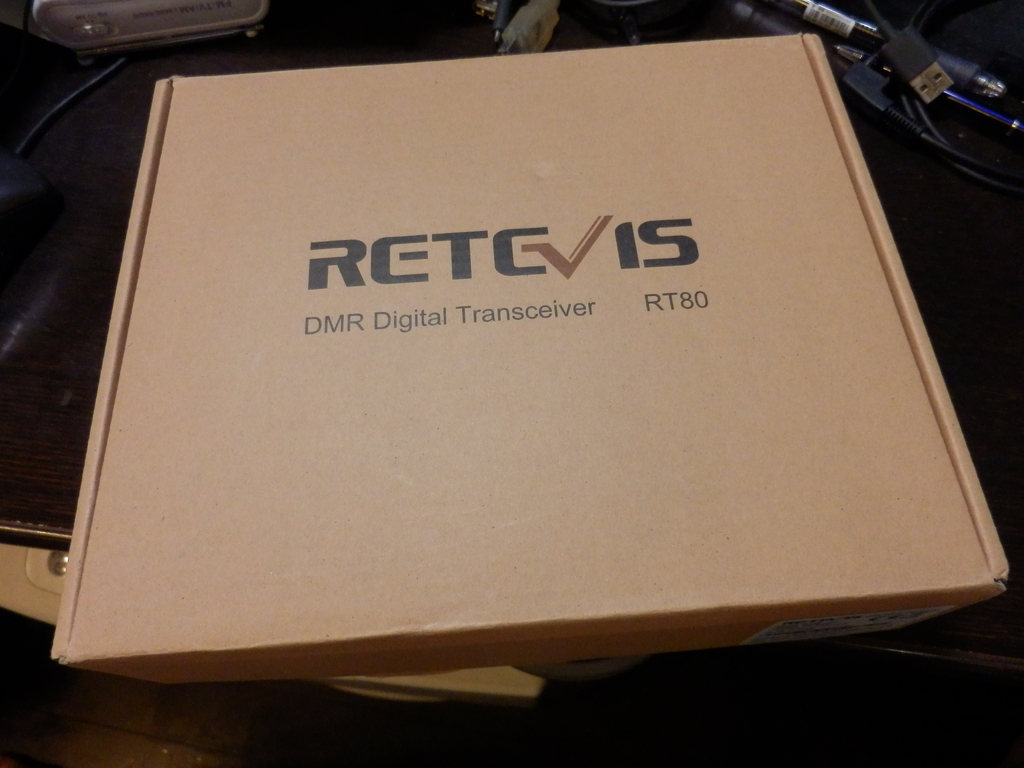
\includegraphics[width=6cm]{img/pa133669.jpg}
 \caption{RT80 のパッケージ}
\end{figure}

モノさえ届けばこちらのもの。この後にやることはただ一つ、分解 (と解析) です。特殊ドライバさえあれば簡単にケースを開けることができます。

\begin{figure}[H]
 \begin{minipage}[t]{0.5\hsize}
  \centering
  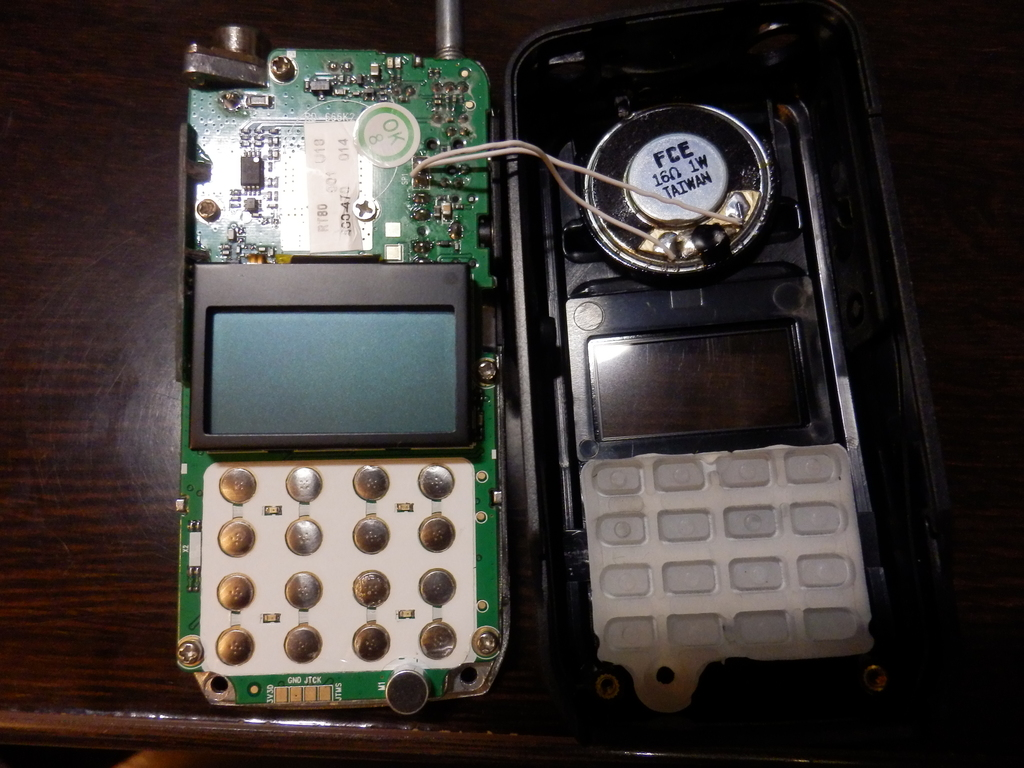
\includegraphics[width=6cm]{img/pa133670.jpg}
  \caption{}
 \end{minipage}
 \begin{minipage}[t]{0.5\hsize}
  \centering
  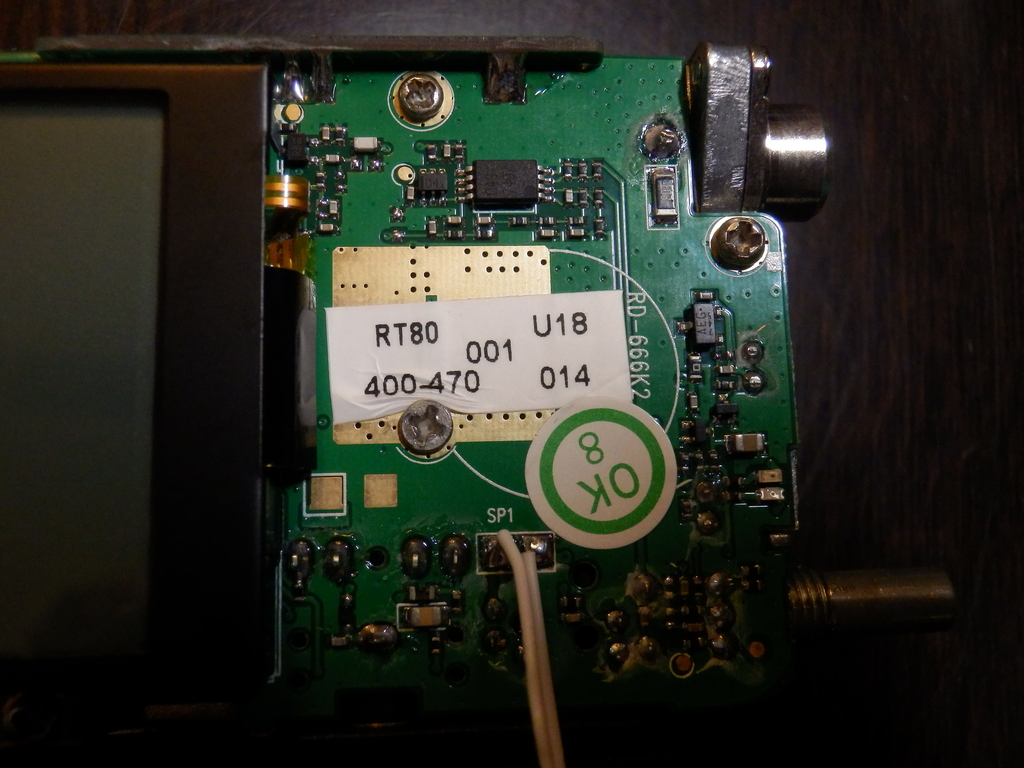
\includegraphics[width=6cm]{img/pa133671.jpg}
  \caption{}
 \end{minipage}
\end{figure}

問題はこの次。メインボードを拝むには、MD-380 の分解\footnote{\url{http://md380.blogspot.com/2016/09/tytera-md-380-teardown.html}}と同様にアンテナ端子の半田を外す必要があります。しかし PTT 周りの基板は付けたままで問題ありません。分解さえできてしまえば、あとは基板のあちこちをデジカメで撮るだけです。撮った画像を Image Composite Editor\footnote{\url{https://www.microsoft.com/en-us/research/product/computational-photography-applications/image-composite-editor/}} でつなぎ合わせ、いくつかの写真にしてみました。

\begin{figure}[H]
 \centering
 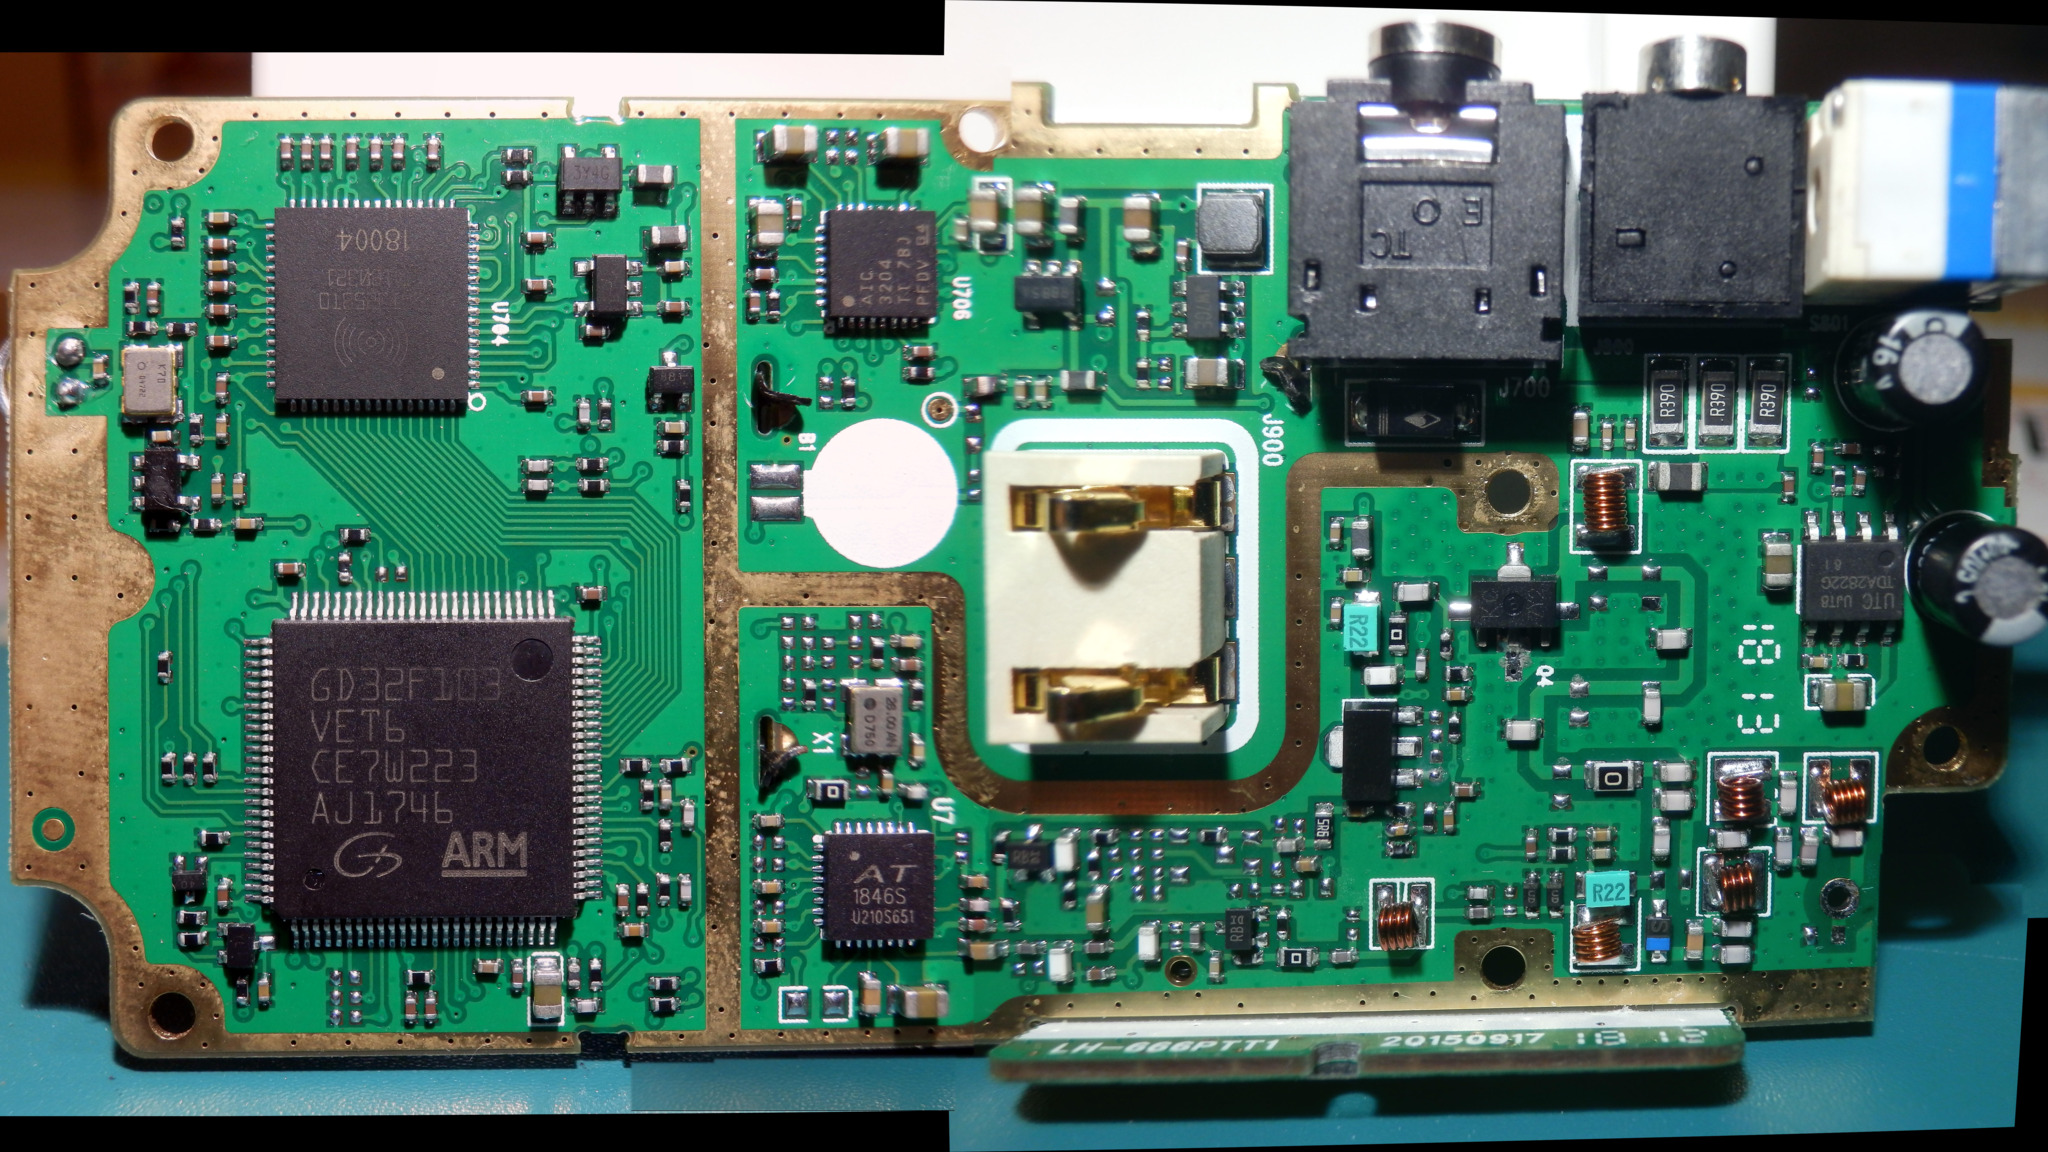
\includegraphics[width=15cm]{img/pa163690_stitch.jpg}
 \caption{RT80 メインボード (1) 全体}
\end{figure}

\begin{figure}[H]
 \centering
 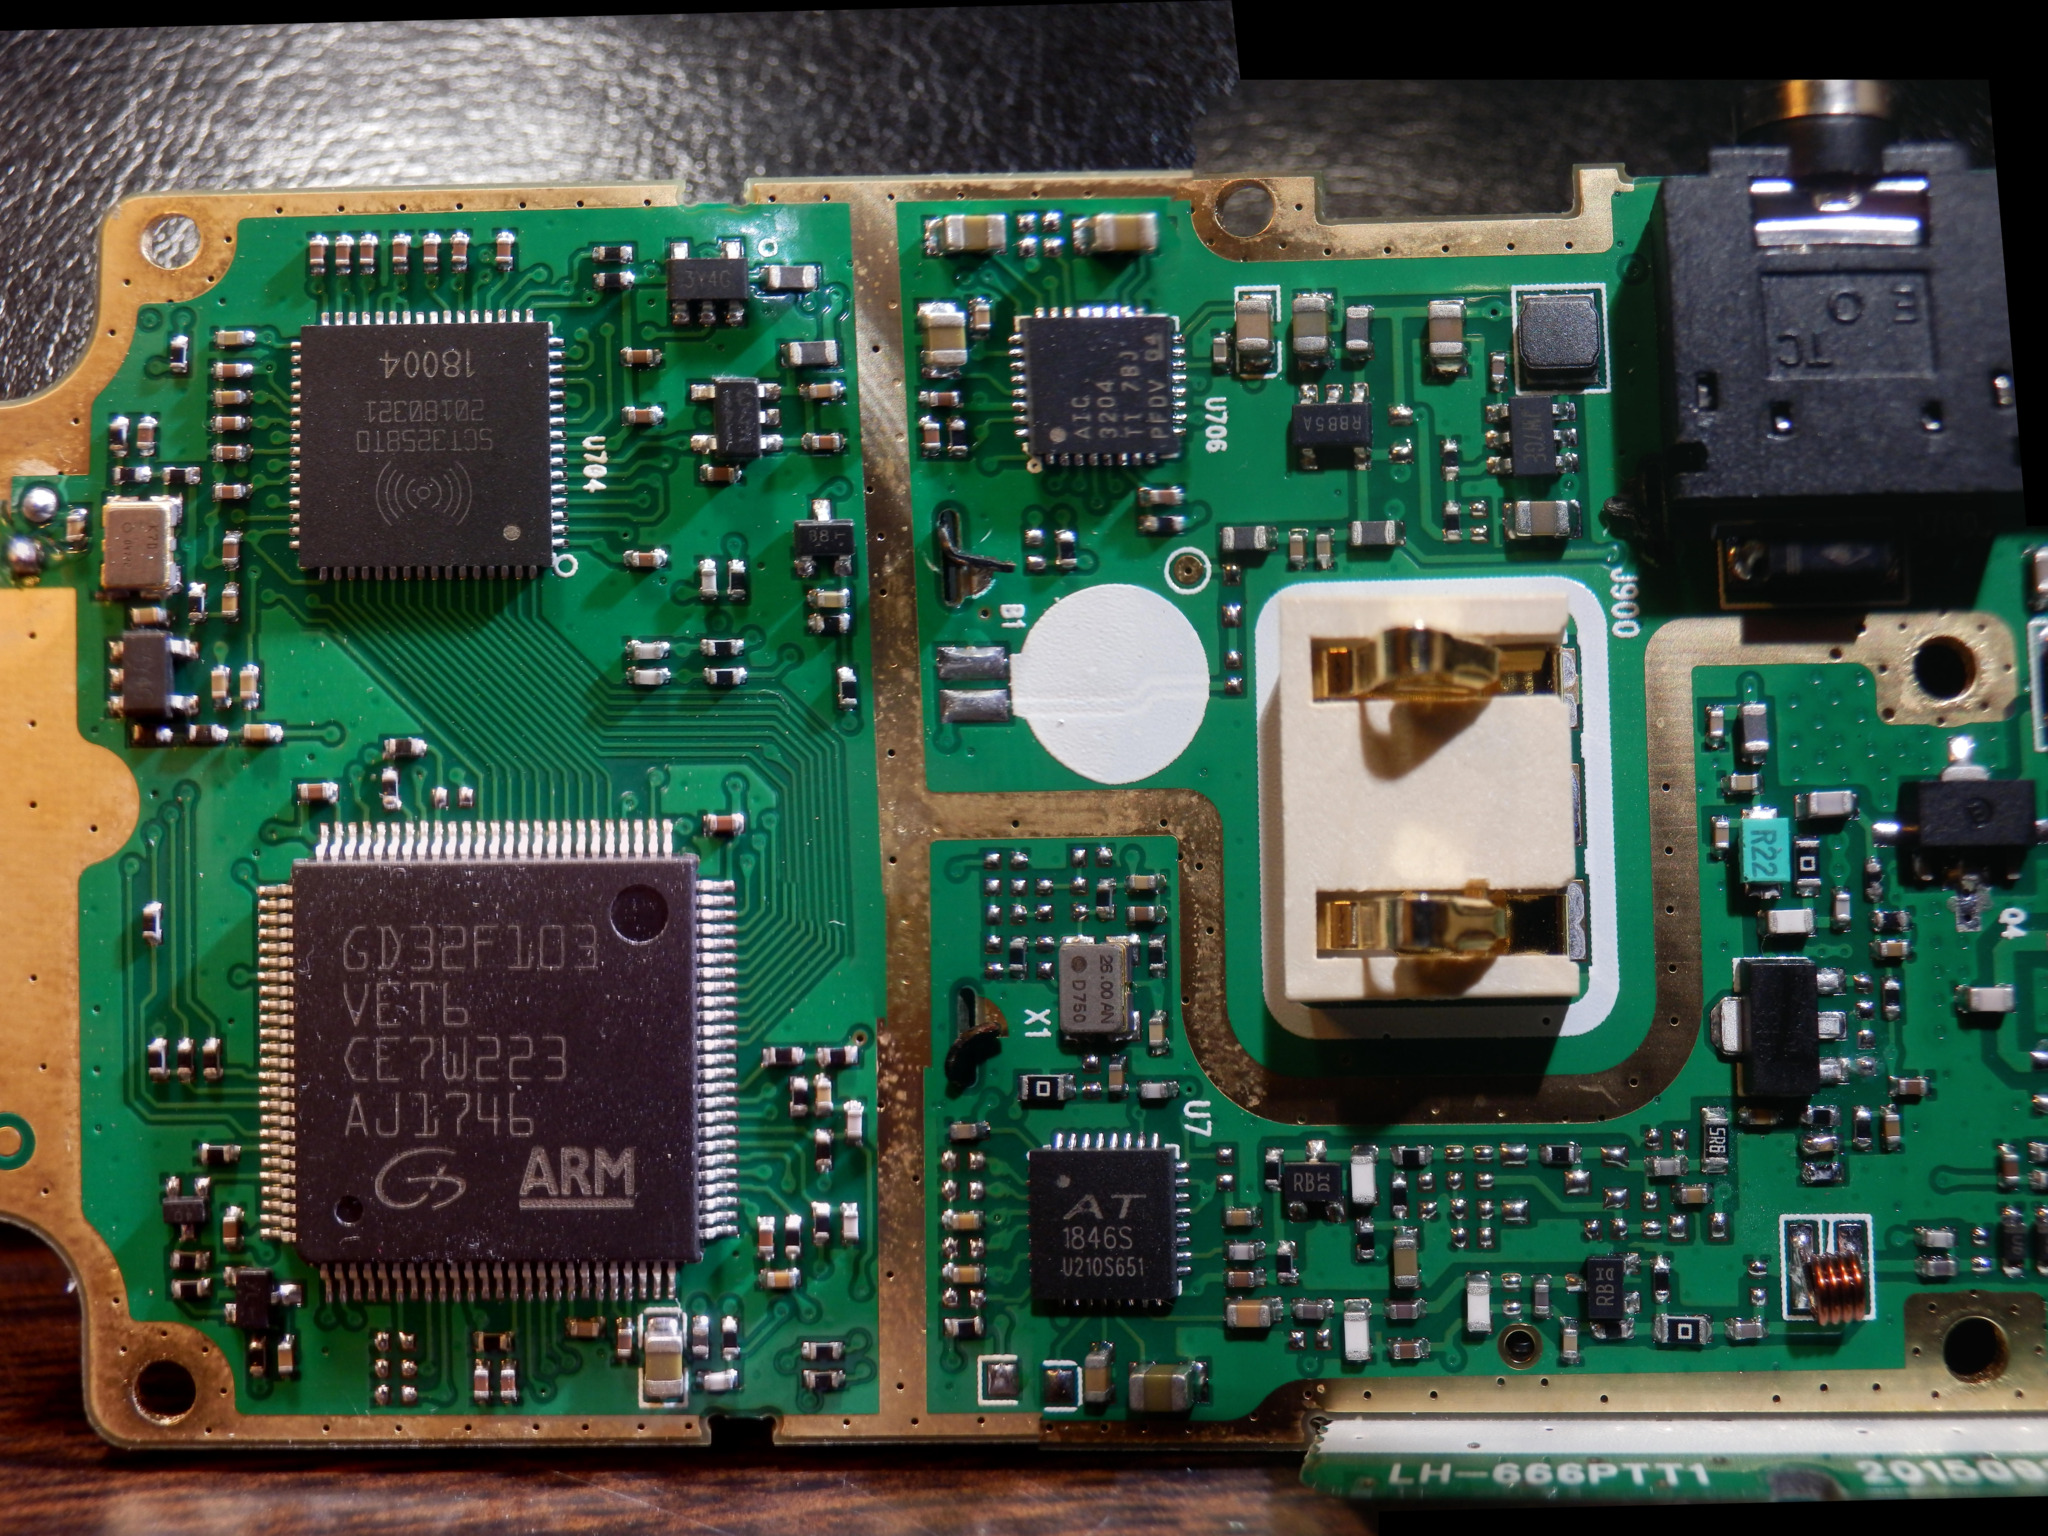
\includegraphics[width=10cm]{img/pa143682_stitch.jpg}
 \caption{RT80 メインボード (2) プロセッサ周辺}
\end{figure}

\begin{figure}[H]
 \begin{minipage}[t]{0.4\hsize}
  \centering
  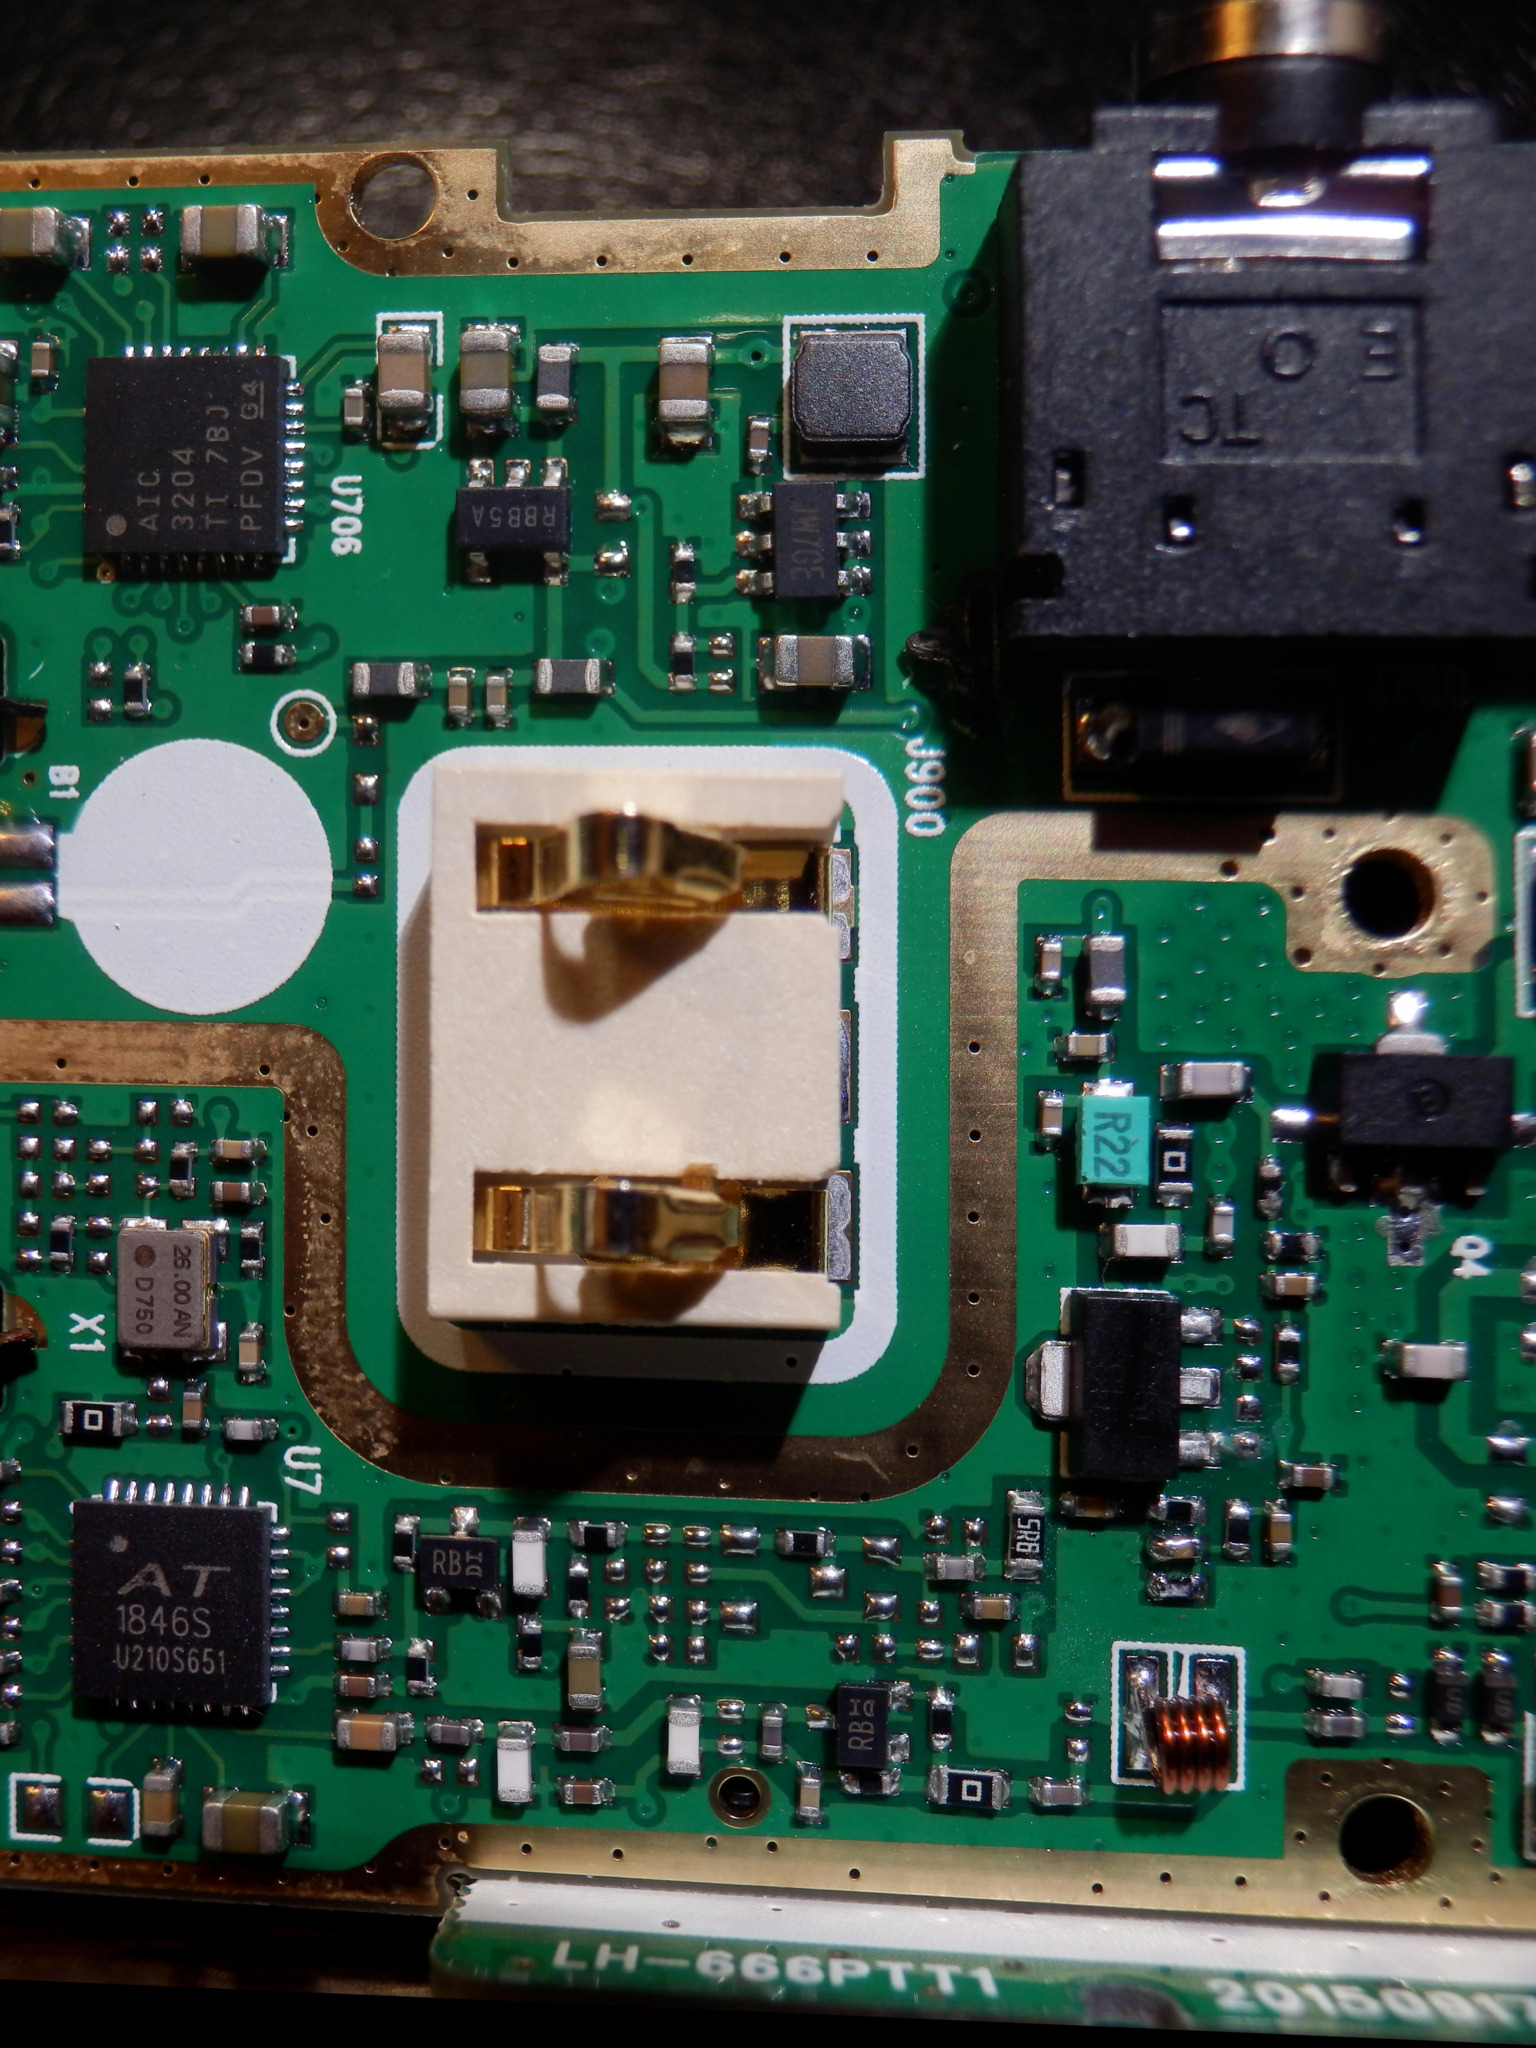
\includegraphics[height=7.5cm]{img/pa143684_stitch.jpg}
  \caption{RT80 メインボード (3) トランシーバ周辺}
 \end{minipage}
 \begin{minipage}[t]{0.6\hsize}
  \centering
  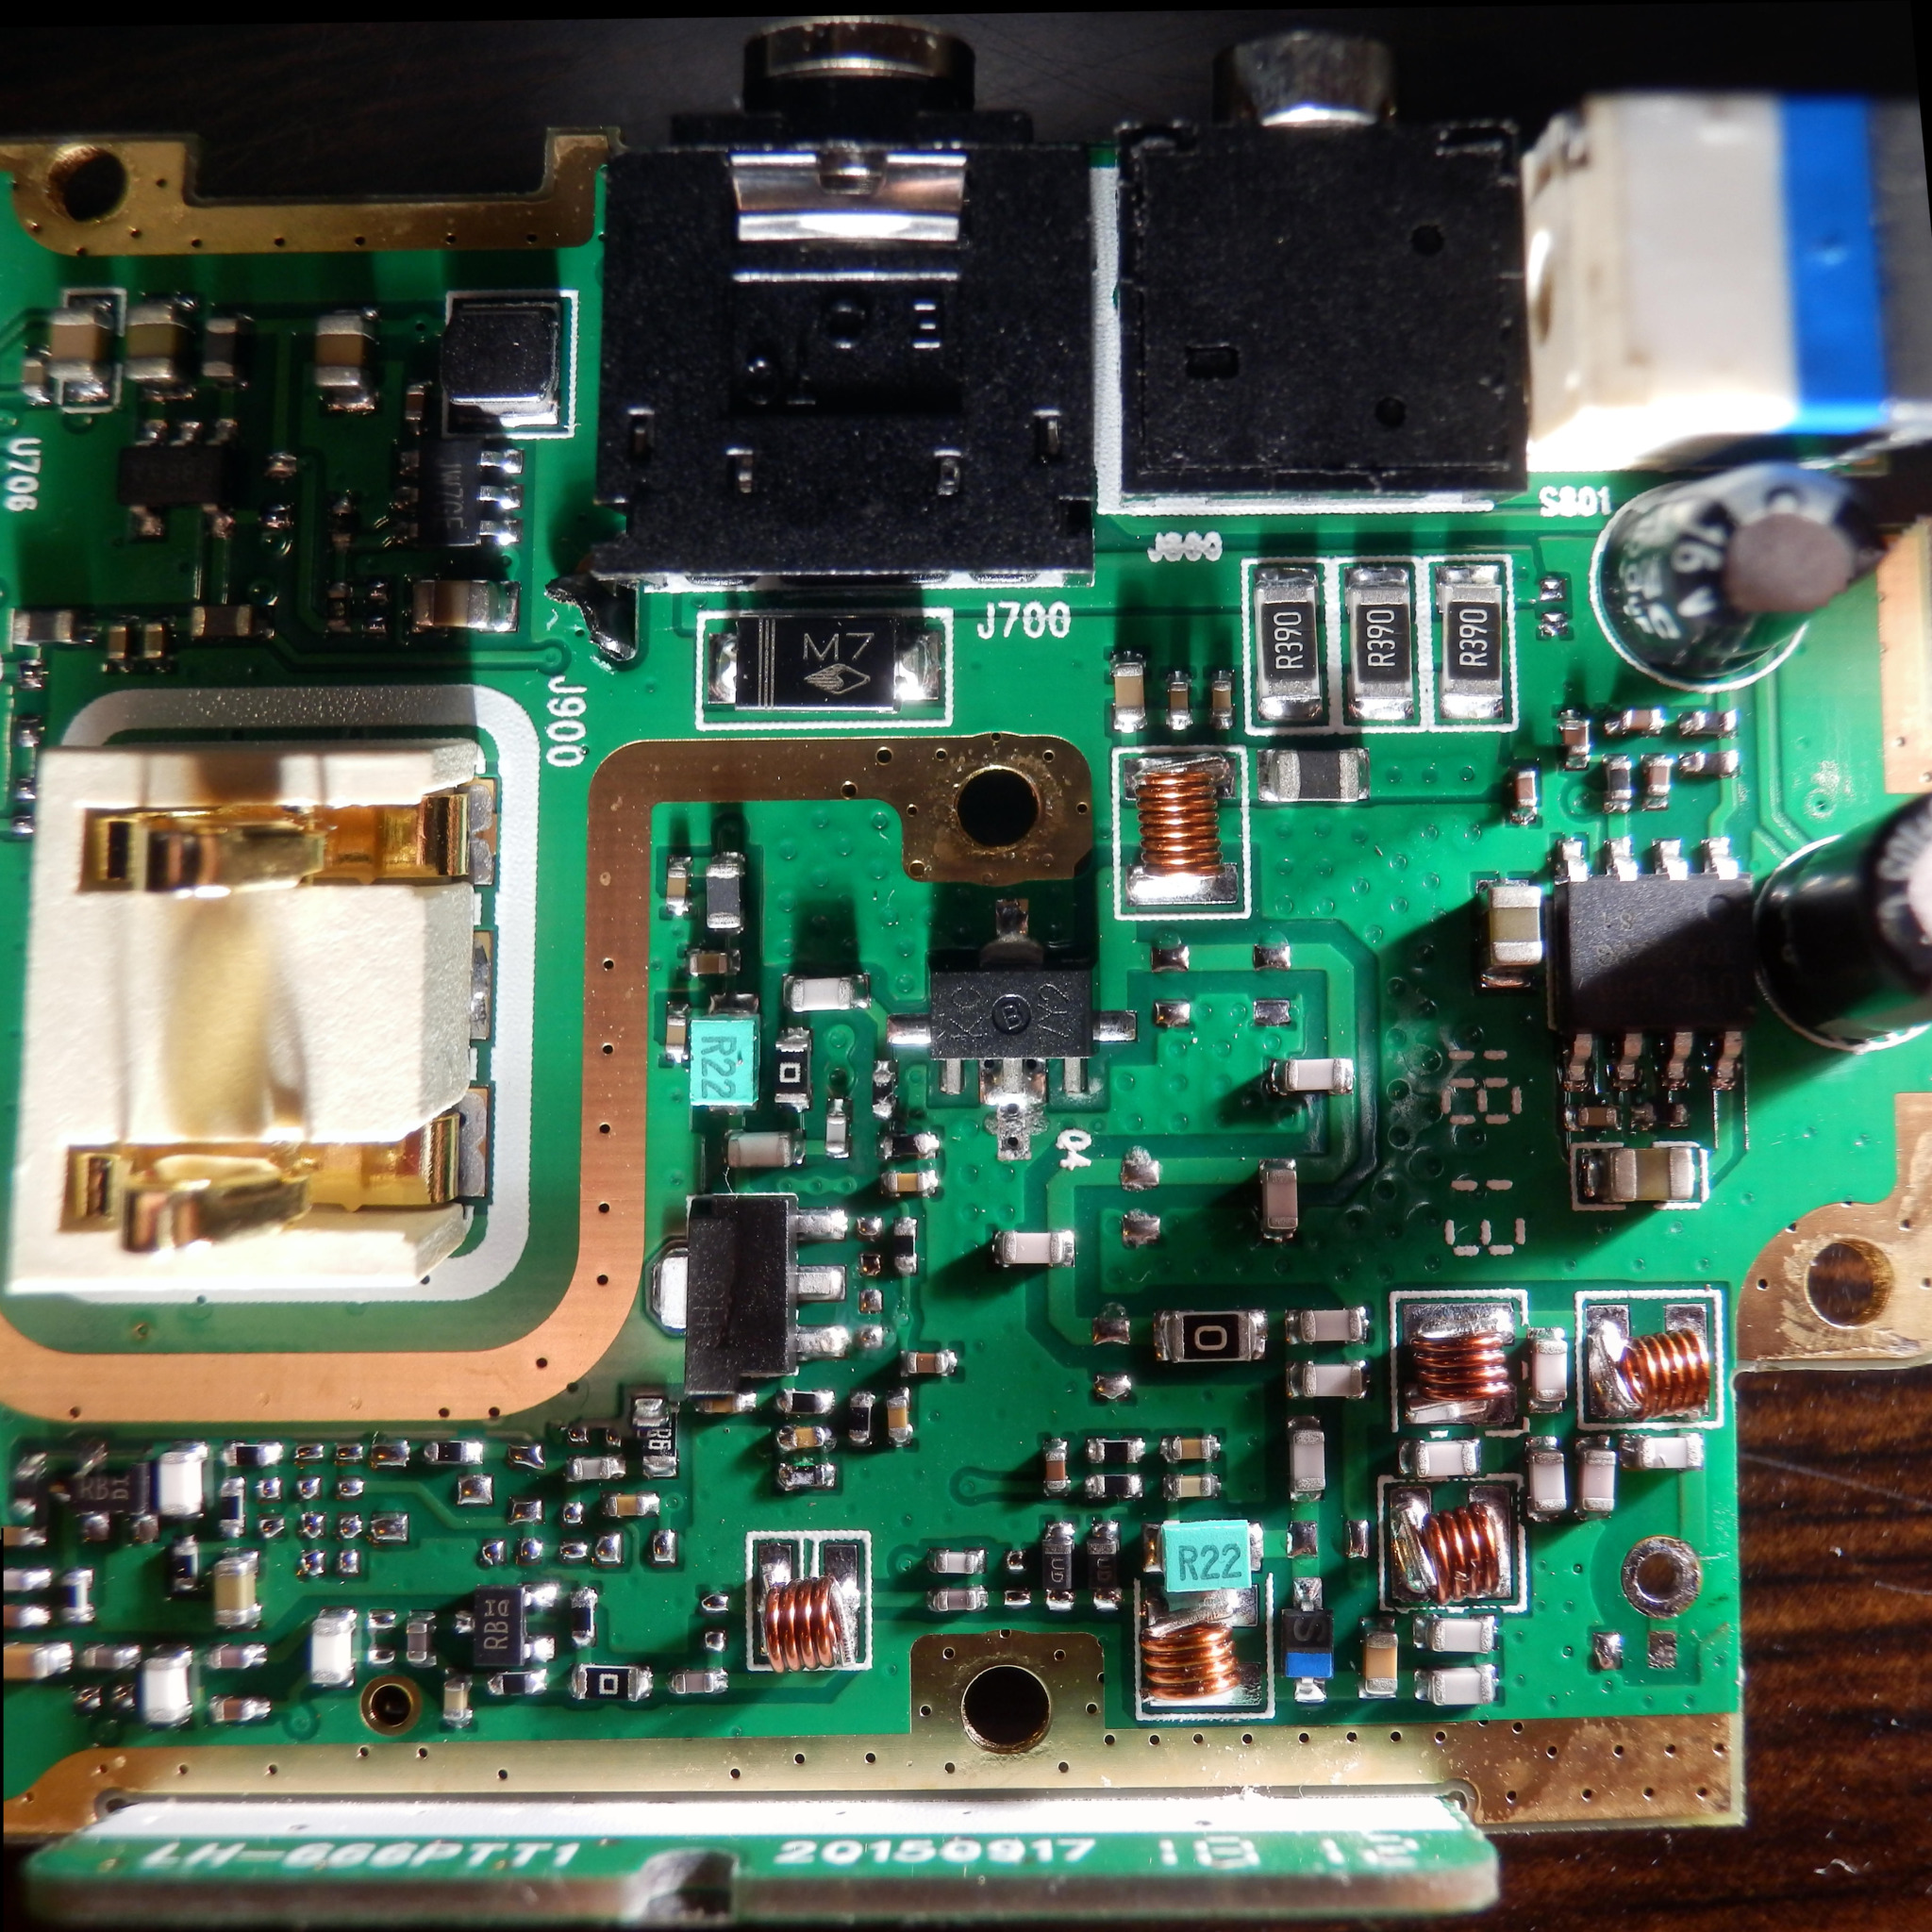
\includegraphics[height=7.5cm]{img/pa143686_stitch.jpg}
  \caption{RT80 メインボード (4) 終段周辺}
 \end{minipage}
\end{figure}

\section{部品を調べて書類を書こう}

イマドキの無線機に使われている部品は非常に小さく、ルーペを使ってもマーキングを読むのに苦労します。また、角度を変えてデジカメで何枚か撮っても印字が薄くて読むのに難儀する部品もあります。基板上の部品のマーキングを拾い、Baofeng UV-5R/UV-3R や YAESU FT-65 で採用している RDA1846S(AT1846S)→2SC3356→2SK3078→RQA0009 という構成から大きく外れることはないだろうと仮定して調べた結果、以下のようになりました。

\begin{description}[style=nextline]
 \item[SCT3258TD] SICOMM SCT3258 dPMR/DMR base band processor\footnote{\url{http://www.sicommtech.com/en/products/sct3258.html}} 
 \item[AT1846S] AUCTUS AT1846S single-chip transceiver%\footnote{\url{http://www.auctus.cn/enindex/ptshow/id/2.html}}
 \item[GD32F103VET6] GigaDevice GD32F103 ARM Cortex-M3 microcontroller\footnote{\url{https://www.gigadevice.com/products/microcontrollers/gd32/arm-cortex-m3/mainstream-line/gd32f103-series/}}
 \item[AIC3204] Texas Instruments TLV320AIC3204 stereo audio CODEC\footnote{\url{https://www.ti.com/product/TLV320AIC3204}}
 \item[RB DI] KEC KTC3770U\footnote{\url{http://www2.kec.co.kr/data/databook/pdf/KTC/Eng/KTC3770U.pdf}}
 \item[H3 0937] HERO HE3078 (2SK3078互換)
 \item[KC 7Y2] MITSUBISHI RD02LUS2\footnote{\url{https://www.mitsubishielectric.com/semiconductors/content/product/highfrequency/siliconrf/discrete/rd02lus2.pdf}}
\end{description}

KTC3770U, HE3078, RD02LUS2 を突き止めるのには時間がかかりました。KTC3770U, HE3078 は「\foreignlanguage{schinese}{丝印} H3 SOT89」や「\foreignlanguage{schinese}{丝印}RB sot」のように中国語で検索しないと見つけることができず、RD02LUS2 はそれでも見つからなかったので Retevis の Facebook ページ\footnote{\url{https://www.facebook.com/retevis/}}からオンラインチャットで聞き出しました。

ここまで入手した情報を元に、作成した RT80 の送信機系統図がこちらです\footnote{当初はAT1846S→\underline{KTC3770U→KTC3770U}→HE3007としこれを申請に使っていましたが、トランジスタ数を考えるとAT1846S→\underline{KTC3770U}→HE3007とした方が適切と判断し、修正した図を掲載しています。}。

\begin{figure}[H]
 \centering
 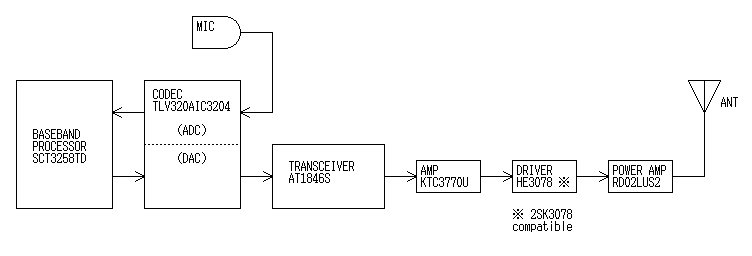
\includegraphics[width=15cm]{img/rt80-2.png}
 \caption{RT80 送信機系統図}
\end{figure}

工事設計書も作成します。RT80 の申請は電子申請Liteではなく紙で行いました (理由は後述)。
\begin{description}[style=nextline]
 \item[発射可能な電波の形式及び周波数の範囲] F2D F3E F7W 430MHz 
 \item[変調方式] F2D, F3E 数値演算型周波数変調 \newline
   F7W 数値演算型四値周波数偏移変調 
 \item[終段管 (名称×個数・電圧)] RD02LUS2 × 1 個 7.4V 
 \item[定格出力] 5W
\end{description}
終段管に印加する電圧は、RT80 のバッテリー (7.4V) と同じです。メーカーの謳い文句では RD02LUS2 は 470MHz, 2W, 3.6V の MOS FET となっており、こんな電圧を印加したら壊れてしまうのではないかと思いデータシートを確認してみました。7V 印加時に 6W 程度の出力が得られるというグラフがあったこと、および絶対最大定格内ではあるため、おかしな使い方ではなさそうです\footnote{とはいえ、何故 RQA0009 を使わなかったのかという疑問は残ります。}。

送信機系統図と工事設計書が揃い、変更申請書と保証認定の願書を用意して JARD に送ってみたところ、「新スプリアス規定に合致する事の確認が取れるデータが必要です」という返事が来ました。問い合わせてみると、FCC 向けの測定方法と日本向けの測定方法は異なっているため、FCC ID を取っているという理由だけでは受け付けることができないそうです。

\section{JARD の測定器室を利用しよう}

無線機が新スプリアス基準を満たしているかどうかはスペクトラムアナライザによる測定が必要になりますが、安価なものが出てきているとはいえ高価な測定器であることは間違いがありません。そこで、JARD の測定器室\footnote{\url{https://www.jard.or.jp/gitekininsho/measuring_instrument_service/}}を利用します。
\begin{figure}[H]
 \centering
 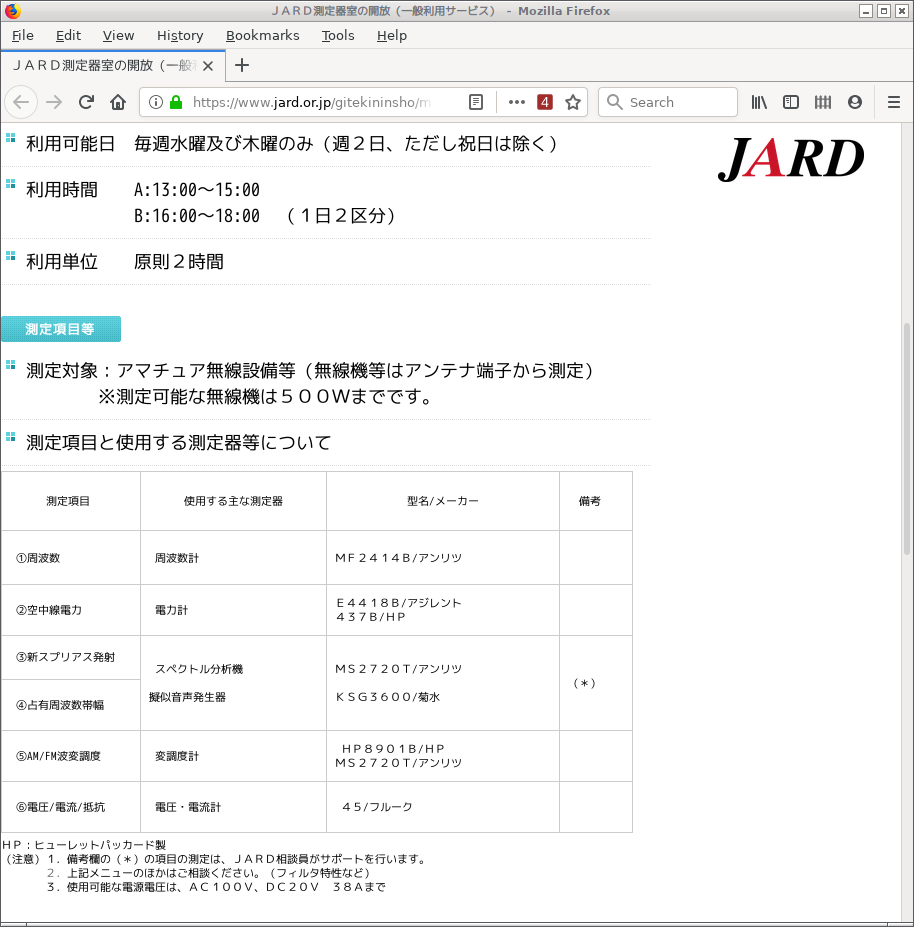
\includegraphics[width=15cm]{img/jard-measureroom.png}
 \caption{JARD 測定器室の利用案内}
\end{figure}
詳細な情報は、とちぎBS140さんのblog\footnote{\url{https://tochigibs140.exp.jp/amateurradio/measuring_instrument_service_report}}が参考になります。RT80 のようなハンディ機の測定を行う場合は、以下のような準備が必要になります。
\begin{itemize}
 \item JARD 測定器室の開放 申込ページ\footnote{\url{https://e-application.jard.or.jp/reservation/}}から申し込みを行う
 \item 申し込み後、受付メールが来るのでこれを印刷する
 \item 当日は以下の機材を持参する
  \begin{itemize}
   \item 印刷した受付メール
   \item 測定器室の利用料 (現金)
   \item USB メモリ (スプリアス測定結果保存用)
   \item 測定対象となる無線機
   \item その他必要なもの (電源ケーブルなど)
  \end{itemize}
\end{itemize}
測定する前に準備しておくべきことや、疑問となることがあれば予めメールで質問しておくと良いでしょう。RT80 に関しては、以下の準備を行って持参しました。
\begin{itemize}
 \item バッテリーをフル充電する
 \item DMR/Analog (25kHz) 各モードにおいて、周波数 435.0000MHz、最大出力を予めメモリしておく
 \item TOT (Time Out Timer) は無効化しておく
\end{itemize}
RT80 はハンディ機 (バッテリー駆動) なので電源ケーブルは無く、また擬似音声発生器の音響出力はスピーカーみたいなものを使ってマイクに入れるためこの部分の接続ケーブルは不要でしたが、テストする無線機によってはこれらのケーブルも持参する必要があるでしょう。無線機と測定器と接続するためのリバース SMA からの変換コネクタ (SMA/M/N/BNC) は持っていれば持参するように言われますが、持っていなければ借りることができます。

測定自体は JARD の担当者が行ってくれるので、こちらは指示に従って PTT、モード (DMR/Analog) を切り替える操作を行うだけです。2 台の RT80 を測定してみましたが、どちらとも新スプリアス基準を満たしていることを確認しました。

RT80 の変更申請は電子申請 Lite ではなく紙で行っており、一旦取り下げた際に戻ってきた申請書一式も持参しました。申請書の書き方で何か問題点がないか相談するつもりでいたのですが、これについては問題はなさそうであること、そして「折角だから申請してはどうか」とのアドバイスでその場で提出してきました。

\section{そして}

JARD に書類を提出してから、二〜三週間くらいの時間で免許状を手にしています。手間はかかりましたが、手順を踏めば海外製の無線機でも (基準を満たしていれば) 日本国内で利用可能なことが分かりました。

RT80、DMR 機としての基本的な機能は持っていますが不満がない訳ではありません。MD-380 のような改造ファームウェアを使用して発信者のコールサインを表示するようなことはできませんし、SMS 周りも MD-380 との互換性は無いようで BrandMeister 越しでもメッセージをやりとりすることができません。とはいえ、MD-380 より軽く、操作性の良い点は非常に気に入っています。

これを書いている時点だと Baofeng DM-1801 の方が RT80 よりも安く、AliExpress では \$55 程度の価格で出ています。他にも魅力的な DMR 機がいくつかあり、機会があれば挑戦してみたいと考えています。

\chapter{USB 非対応の JumboSPOT をパソコンで使うために}

\section{USB 非対応でも大丈夫です}

本文では USB 接続に対応した JumboSPOT をパソコンに接続するようにしていますが、入手性があまり良くないため、ここで USB 接続に非対応の JumboSPOT を入手した場合について補足します。

\section{電源と UART さえ繋げば動きます}

JumboSPOT は、Raspberry Pi の 40 ピン GPIO 端子に装着して使用するように作られています。しかし JumboSPOT が実際に使用するのは電源 (5V/3.3V/GND) および UART (TXD/RXD) だけなので、然るべきものを用意すれば Raspberry Pi 以外でも動作させることが可能です。UART については USB-UART アダプタで対応し、電源については USB から 5V を取り、ここから 3.3V をレギュレータで生成すれば良いでしょう\footnote{USB-UART アダプタから 3.3V を取る方法もありますが、アダプタによっては電源容量が不足する可能性もあるため、ここではレギュレータを使用しています。}。

USB-UART は CH340E を搭載したアダプタを使用しましたが、以下の条件を満たしていればどのようなコントローラを搭載していても動作すると思われます。

\begin{itemize}
 \item 5V の電源端子がある
 \item RXD/TXD 信号を 3.3V で入出力できる
 \item OS が USB-UART コントローラに対応している (ドライバを持っている)
\end{itemize}

配線自体は難しいものではなく、対応する端子に対応する信号や電圧を接続するだけです。レギュレータについては、AliExpress で売られていた DD0403MA 搭載 LDO モジュールを使用しましたが、3.3V を生成し十分な電源容量が得られれば何でも構いません。雑な図ですが、こんな感じになるでしょうか。

\begin{figure}[H]
 \begin{minipage}[t]{0.5\hsize}
  \centering
  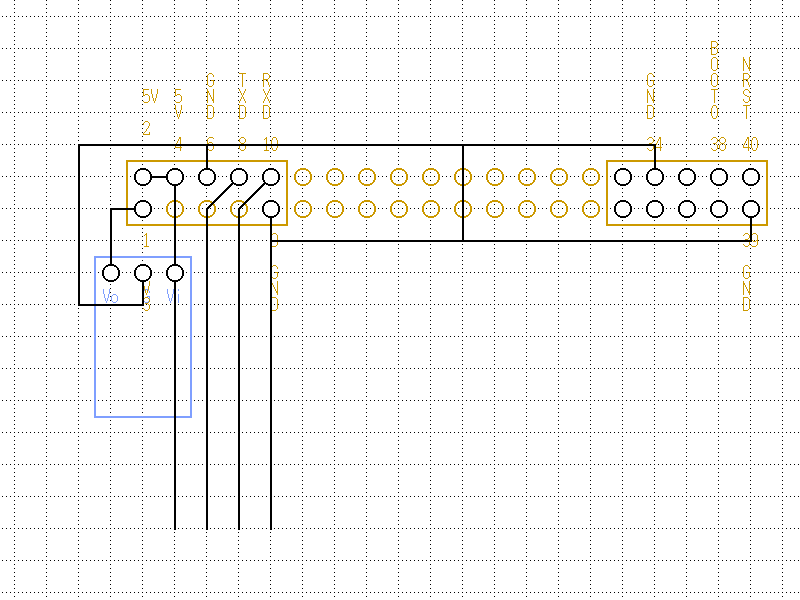
\includegraphics[width=6cm]{img/conn.png}
  \caption{配線図 (部品面)}
 \end{minipage}
 \begin{minipage}[t]{0.5\hsize}
  \centering
  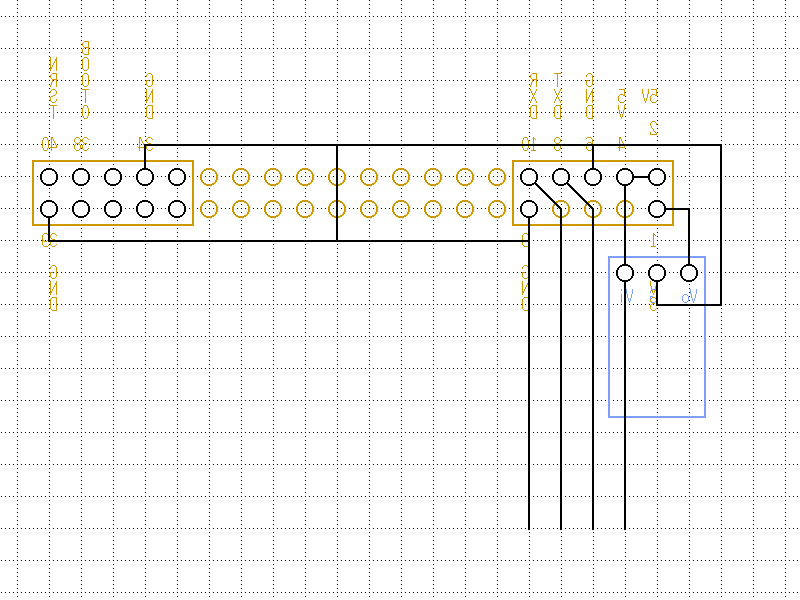
\includegraphics[width=6cm]{img/conn_r.png}
  \caption{配線図 (半田面)}
 \end{minipage}
\end{figure}

\section{実際に作ってみました}

ピンが曲がっていたり、ハンダ付けもあまり上手い訳では無いのですが、製作例です。JumboSPOT ファームウェア書き換え用のコネクタ (Rasperry Pi のピン 38, 40 に対応する部分) も実装していますが、これは省略しても構いません。

\begin{figure}[H]
 \begin{minipage}[t]{0.5\hsize}
  \centering
  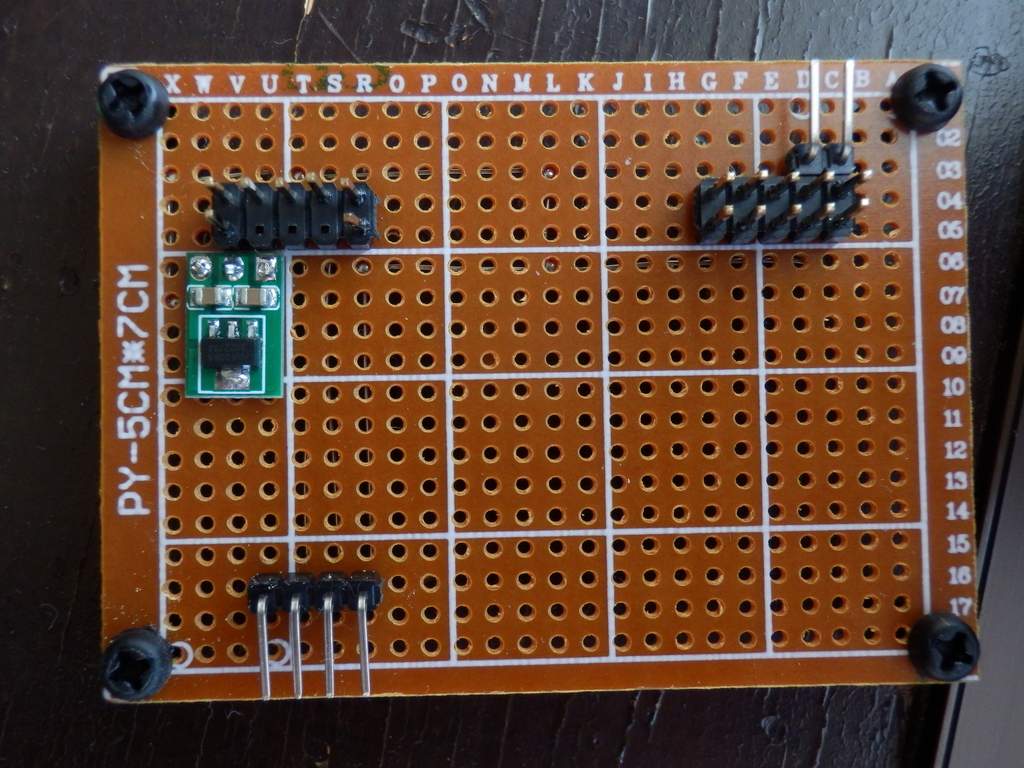
\includegraphics[width=6cm]{img/p2234402.jpg}
  \caption{組立例 (部品面)}
 \end{minipage}
 \begin{minipage}[t]{0.5\hsize}
  \centering
  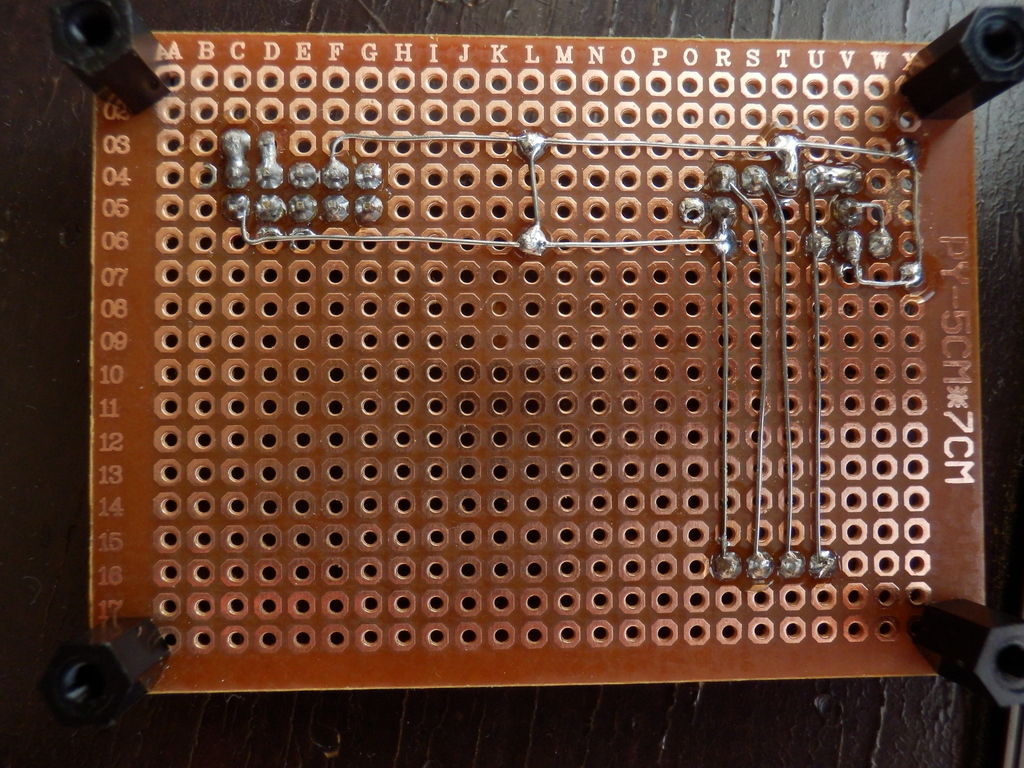
\includegraphics[width=6cm]{img/p2234403.jpg}
  \caption{組立例 (半田面)}
 \end{minipage}
\end{figure}

JumboSPOT を搭載して USB-UART を接続し、PC 上の MMDVMHost から制御できることも確認しています。

\begin{figure}[H]
 \begin{minipage}[t]{0.5\hsize}
  \centering
  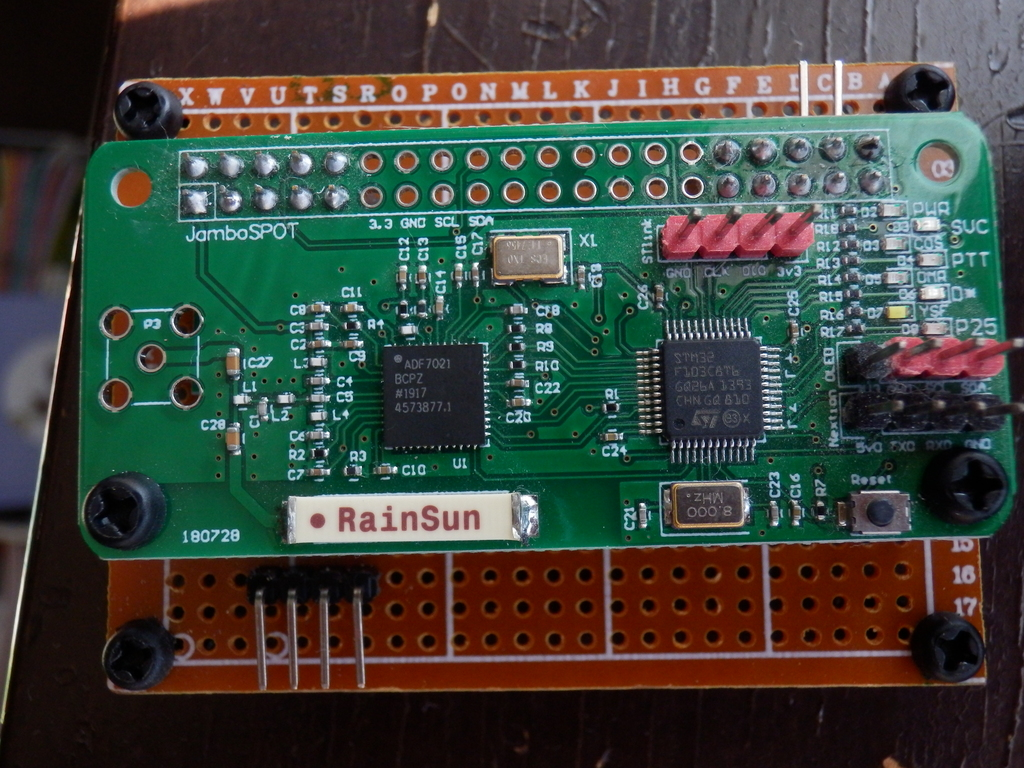
\includegraphics[width=6cm]{img/p2234401.jpg}
  \caption{JumboSPOT 装着時の状態}
 \end{minipage}
 \begin{minipage}[t]{0.5\hsize}
  \centering
  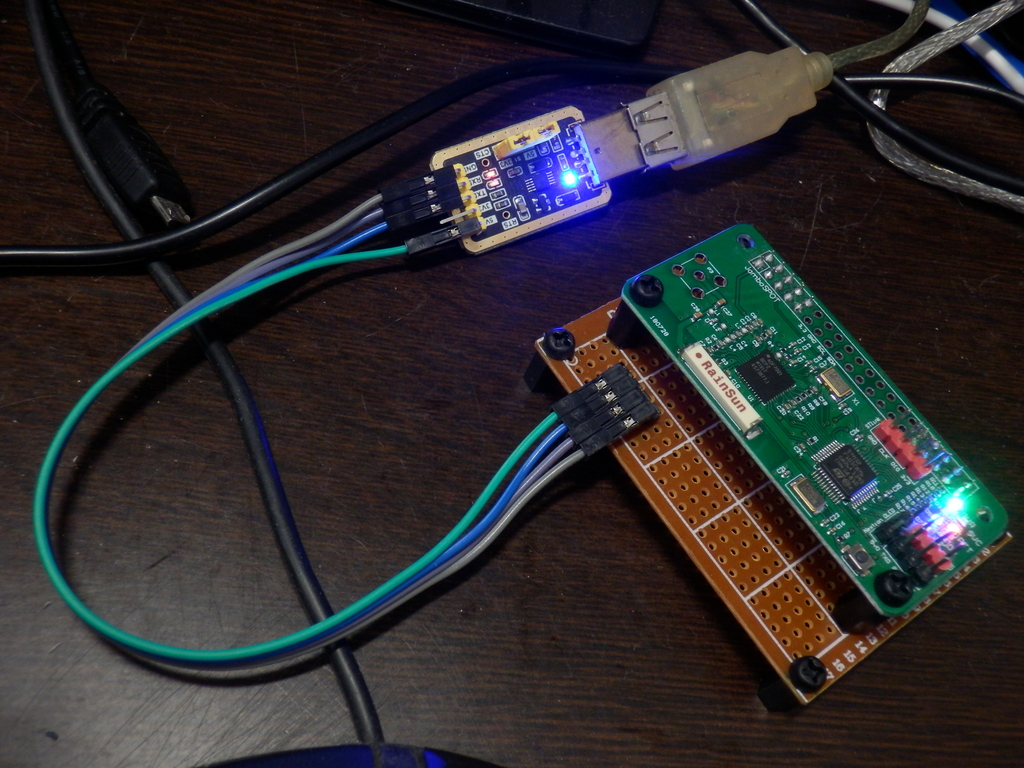
\includegraphics[width=6cm]{img/p2234409.jpg}
  \caption{動作中の様子}
 \end{minipage}
\end{figure}

なお、USB 接続に対応した JumboSPOT は \verb+/dev/ttyACM0+ に接続されますが、USB-UART を使用して接続した場合は \verb+/dev/ttyUSB0+ となる場合もあるので注意が必要です\footnote{USB-CDC (Communication Device Class) に準拠したデバイスでは \tt{/dev/ttyACM0} となりますが、そうでない場合は \tt{/dev/ttyUSB0} となります。}。

\section{参考文献}
\begin{description}[style=nextline]
 \item [JumboSPOT+bluetooth] \url{http://jg3ebb.mydns.jp/html/art/00089.html}
\end{description}

\end{document}
